\documentclass[a4paper,11pt]{report}

\usepackage[headheight=13.7pt]{geometry}
\usepackage[scaled=0.91]{helvet}
\usepackage{courier}
\usepackage[color,relax]{composestar}
\usepackage{chngpage}
\usepackage[numbers]{natbib}
\usepackage[draft]{fixme}
\usepackage{calc}
\usepackage{amsmath}
\usepackage{longtable} %needed for the tables.
\usepackage{array} % for the {IcI}-part in tables
\usepackage{fancyhdr} % The header and footer package
\usepackage[Lenny]{fncychap} % fancy chapter headings
\usepackage{picins, graphicx}
\usepackage{wrapfig} % wrap figure around text -> replacemnt of picins?
\usepackage{multicol}

\usepackage[
%   	colorlinks=true,%
   	bookmarksnumbered=true,%
   	bookmarksdepth=3,%
   	linktocpage=true,%
   	plainpages=false,%
   	pdfpagelabels=true,%
   	pdfstartview=FitH%
]{hyperref}

\renewcommand{\sectionautorefname}{section}
\renewcommand{\subsectionautorefname}{\sectionautorefname}
\newcommand{\subfigureautorefname}{\figureautorefname}

\graphicspath{{./}{./images/}{./images/logos}}

% Define grammar language in listings.
\lstdefinelanguage{ebnf}{%
  %otherkeywords={=, (, ), [, ], \{, \}, -, ;},%
  literate={~}{$\sim$}1,
  sensitive=true,%
	morestring=[b]",%
	morestring=[b]',%
  morecomment=[s][\color{magenta}]{?}{?},%
  morecomment=[s]{(*}{*)}%
}[keywords,comments,strings]
\lstdefinelanguage{antlr}{%
  morekeywords={:, (, ), *, [, ], +, ?, !},%
  literate={~}{$\sim$}1,
  sensitive=true,%
	morestring=[b]",%
	morestring=[b]',%
  morecomment=[l]{//},%
  morecomment=[s]{/*}{*/}%
}

% Listing style with colored keywords in a footnote sized font.
\lstdefinestyle{listingWithNoNumbers}{%
  style=clean,%
  style=color,%
  basicstyle=\footnotesize\ttfamily,%
  tabsize=2,%
  breaklines=true,%
  captionpos=b%
}

\lstset{style=inline}
\lstloadlanguages{[AspectJ]Java,[HyperJ]Java,ComposeStar, ebnf}

\setcounter{tocdepth}{0}

%---------------------------------------------------------------------------------------
% Float env.
%---------------------------------------------------------------------------------------
\setcounter{topnumber}{1}
\setcounter{bottomnumber}{2}
\setcounter{totalnumber}{8} % fill in these float pages
\renewcommand{\textfraction}{0.50}	% allow no text
\renewcommand{\floatpagefraction}{0.4} % small float pages

%---------------------------------------------------------------------------------------
% Chapter on/off counters
%---------------------------------------------------------------------------------------
\newcounter{@comments}
\newcounter{@dotnetcomments}
\newcounter{@javacomments}
\newcounter{@ccomments}
\newcounter{@starlightcomments}
\newcounter{@faq}
\newcounter{@furtherreading}
\newcounter{@pending}

%---------------------------------------------------------------------------------------
% F.A.Q commands
%---------------------------------------------------------------------------------------
\newcommand{\question}[1]{\textit {\textbf {Q:} \xspace #1 \\}}
\newcommand{\answer}[1]{\textbf{A:} \xspace #1 \\}

%---------------------------------------------------------------------------------------
% General
%---------------------------------------------------------------------------------------
% Table settings both from the LaTeX companinion 2nd ed.
\newcolumntype{I}{!{\vrule width 1.7pt}}
\newlength\savedwidth
\newcommand\whline{\noalign{\global\savedwidth\arrayrulewitdh
                            \global\arrayrulewidth 3pt}%
                   \hline
                   \noalign{\global\arrayrulewidth\savedwidth}}

\newcommand{\para}[1]{\textbf{#1}\\}
\newcommand{\subpara}[1]{\textit{\textbf{#1}}\\}
\newcommand{\faq}[1]{\ifthenelse{\value{@faq}= 1}{\section{FAQ and Hints}#1}{}}
\newcommand{\comments}[1]{\ifthenelse{\value{@comments}= 1}{\section{Commentary}#1}{}}
\newcommand{\dotnetcomment}[1]{\ifthenelse{\value{@comments}= 1 \and \value{@dotnetcomments}= 1}
{\subsection{Comments on \Compose*[DotNet]}
  %\begin{wrapfigure} [6] {l} [0pt] {0pt}
  	%\begin{figure}
			%\centering
			%\includegraphics[width = 2.5 cm]{images/logos/DotNet}
		%\end{figure}    
  %\end{wrapfigure}
#1}{}}
\newcommand{\javacomment}[1]{\ifthenelse{\value{@comments}= 1 \and \value{@javacomments}= 1}
{\subsection{Comments on \Compose*[Java]}
  %\begin{wrapfigure} [6] {l} [0pt] {0pt}
  	%\begin{figure}
			%\centering
			%\includegraphics[width = 2.5 cm]{images/logos/java}
		%\end{figure}    
  %\end{wrapfigure}
#1}{}}
\newcommand{\ccomment}[1]{\ifthenelse{\value{@comments}= 1 \and \value{@ccomments}= 1}
{\subsection{Comments on \Compose*[C]}
  %\begin{wrapfigure} [6] {l} [0pt] {0pt}
  	%\begin{figure}
			%\centering
			%\includegraphics[width = 2.5 cm]{images/logos/Cplain}
		%\end{figure}    
  %\end{wrapfigure}
#1}{}}
\newcommand{\starlightcomment}[1]{\ifthenelse{\value{@comments}= 1 \and \value{@starlightcomments}= 1}
{\subsection{Comments on StarLight}
  %\begin{wrapfigure} [6] {l} [0pt] {0pt}
  	%\begin{figure}
			%\centering
			%\includegraphics[width = 2.5 cm]{images/logos/Cplain}
		%\end{figure}    
  %\end{wrapfigure}
#1}{}}
\newcommand{\pending}[1]{\ifthenelse{\value{@pending}= 1}
{\section{Pending Questions}
  %\begin{wrapfigure} [6] {l} [0pt] {0pt}
  	%\begin{figure}
			%\centering
			%\includegraphics[width = 2.5 cm]{images/logos/karel}
		%\end{figure}    
  %\end{wrapfigure}
#1}{}}
\newcommand{\furtherreading}[1]{\ifthenelse{\value{@furtherreading}= 1}{\section{Further Reading}#1}{}}

\newcommand{\turnOn}[1]{\setcounter{#1}{1}}
\newcommand{\turnOff}[1]{\setcounter{#1}{0}}

\newcommand{\mult}{$^{*}$}

%---------------------------------------------------------------------------------------
% Rest
%---------------------------------------------------------------------------------------
%Bibliography
\bibliographystyle{alpha}

\newcommand{\nb}{N.B.\xspace}

% to get rid of the standard US style paragraph indent
\parindent = 0pt
\parskip = 11 pt

\makenomenclature

\renewcommand{\subsubsectionautorefname}{\subsectionautorefname}
\usepackage[draft]{fixme}

\begin{document}
\makenomenclature
\title{\Compose*{} Annotated Reference Manual}
\maketitle

\pagestyle{empty}
\fancypagestyle{plain}{
\fancyhead{}% clear header fields
\fancyfoot{}
}

%\chapter*{Acknowledgments}\label{acknowledgments}%\addcontentsline{toc}{chapter}{Acknowledgments}
\fixme{Write me!}

\vspace{20pt}
\begin{flushright}
\today \\
Enschede, The Netherlands \\
\end{flushright}


\chapter*{Reading guide}
Each chapter of the ARM handles a part of the \Compose* language. In each chapter there is first an abstract of what that particular part of the language should do. 
After that the syntax and the semantics are demonstrated.
The syntax is presented in ISO EBNF \cite{scowen1993ebg}.
How it can be used is shown in the examples.
After that the legality rules and the FAQ are stated.

The how, what, and the design decisions are mentioned in the comments. 
If added there can also be specific platform comments for each \Compose* platform.

When there is more to read about a chapter then this is mentioned in the ``further reading'' section of a chapter.

\tableofcontents
\cleardoublepage 
\listoffigures
\cleardoublepage
\printnomenclature  %[1in]

%\listoffixmes

\cleardoublepage
\pagenumbering{arabic}% Arabic numbering 1, 2, ..

%------------------------------------------------------------------------------------------
%% setting some chapters on/off, 1 means on, the rest off.
%------------------------------------------------------------------------------------------
\turnOn{@comments}
\turnOn{@dotnetcomments}
\turnOn{@javacomments}
\turnOff{@ccomments}
\turnOn{@starlightcomments}
\turnOn{@faq}
\turnOn{@furtherreading}
\turnOn{@pending}

%---------------------------------------------------------------------------------------
% Header and footer
%---------------------------------------------------------------------------------------
% from the LaTeX companion
\pagestyle{fancy} \fancyhf{}
\renewcommand\chaptermark[1]{\markboth{\thechapter\ #1} {}}
\renewcommand\sectionmark[1]{\markright{\thesection\ #1} {}}
\renewcommand\subsectionmark[1]{\markright{\thesection\ #1} {}}
\renewcommand\headrulewidth{0.4 pt}
\renewcommand\footrulewidth{0.4 pt}
\fancyhead{}% clear header fields
\fancyfoot{}
\fancyhead[R]{University Twente}
\fancyhead[L]{\textnormal{\leftmark}}
\fancyfoot[L]{\Compose*{} ARM}
\fancyfoot[R]{\thepage}

\fancypagestyle{plain}{
\fancyhead{}% clear header fields
\fancyfoot{}
\fancyfoot[L]{\Compose*{} ARM}
\fancyfoot[R]{\thepage}
\renewcommand\headrulewidth{0 pt}
\renewcommand\footrulewidth{0.4 pt}
}

\chapter{Glossary}
\paragraph{\Compose*[Java]} Compose*.Java is the Java port of Compose*.
\paragraph{\Compose*[DotNET]} Compose*.Net is the .Net port of Compose*.
\paragraph{\Compose*{} developer} A member of the Compose* team, thus who programs on Compose*.
This term is used to avoid the ambiguous term Compose* programmer.
\paragraph{\Compose*{} user} Somebody who uses Compose*, this does not exclude the
person from being a Compose* developer. This term is used to avoid the ambiguous term Compose* programmer.
\paragraph{Default constructor} A constructor without any argument.

\paragraph{Functional complete} A set of logical operators is functional complete when it can express any operator from
the set~\cite{vanBenthem91}.
So a XOR (exclusive OR) is not in a functional complete set, because 
$A~XOR~B~=~(A~AND~!B)~OR~(!A~AND~B)$. The smallest
functional complete set only contains OR and NOT.

\paragraph{Language independence} Compose* is designed to be used for any language, that gives that Compose*
needs to be language independent. This language in dependency influences Compose* in two ways, first on the
syntax and semantics, and second on the under laying mechanisms. True language independence means that a concern can be added to
an application to a random parent language and it behaves he same as if you would place it in the same application
written in a different parent language. For the syntax and semantics this means that we cannot add primitive types to
Compose*, because for instance \emph{int}, \emph{char}, and \emph{double}, can have different ranges.
These limitations can be solved by
automating some conversions, for instance we could introduce our own primitive type \emph{i} which is an integer
of 32 bits, then we can transform this primitive to the primitive value we want by creating a conversion method in
Compose*. However for every work around in the language applies that it is just more code and even more important
that it solves the problem for most of the cases, but is would cause errors in a small number of situations.
For instance we go further with our primitive i, we find ourselves in the situation that this idea only works if the
application stays on one platform and one parent language, if we would import a library then we cannot say for certain
to what primitive type we must convert. So if we apply the our own defined primitives we limit the use of the parent language,
which is something we do not want.

This gives that there are a few basic comments on language independence which are common for all the parts of the
Compose* language:

\begin{itemize}[noitemsep]
\item Keywords from parent languages have language specific meanings, that means that we cannot use them
directly in Compose*.
\item The things that are language independent are Objects, Methods, Packages, and Annotations. However these
might not be available in every language, for instance C does not know Objects and Annotations are not common for all
languages.
\item Workarounds with conversion mechanisms might work, but probably it conceptual not sound or you limit
yourself in another way.
\item If something, for example an integer is 32 bit, in most languages, say Java, C\#, C++, Delphi, then it dos not mean
that it can be made language independence. There is probably one language around where the integer is not 32 bit.
\end{itemize}

\paragraph{Signature of a class} There are various definitions of the signature of a class, the one used in \Compose* is
that the signature of a class is the collection of signatures of the methods of the class. The signature of a class
is the name, return type, and the list of parameter types. The signature of the class in \autoref{glos::signature}
is \{\emph{Sting getName, void setBirthDate(Date), void setBirthDate(String)} \}.

\begin{lstlisting}[caption={Example class in Java},label=glos::signature,float=h,language=Java,style=listing]
public class Person{
	public String getName(){}
	public void setBirthDate(Date date){}
	public void setBirthDate(String date){}
}
\end{lstlisting}

\paragraph{Base language} \Compose* is an extension to other programming languages, the base language is the language
that gets extended. So for \Compose*[Java] the programming language Java is the parent language.

\paragraph{Wild card} The used term for the `*' token, whereas it normally means everything, it means in \Compose*
ignore.
% ARM concern entry
\chapter{Concern} \label{chapter:concern}
Concerns are the distinctive building blocks of a \Compose* application, in addition to the building blocks of the base language. Conceptually concerns are an extension to classes.
Concerns are declared in files with a \emph{.cps} extension.

A concern has three different parts: zero or more filter modules, an optional superimposition part, and an optional implementation part. 
The filter modules are superimposed on classes by the filter module binding field of the superimposition. 
The implementation part contains language dependent code of the concern.

\section{Syntax}
\begin{lstlisting}[caption = {Concern syntax}, label = lst::ARM:concern:syntax, style = listing, language = {ebnf}, float = tpb]
Concern = 'concern' Identifier [ConcernParameters] ['in' Namespace] ConcernBlock;
ConcernParameters = '(' Identifier ':' Type {',' Identifier ':' Type } ')';
Type = Fqn;
Fqn = Identifier {'.' Identifier};
Namespace = Fqn;
ConcernBlock = '{' {FilterModule} [SuperImposition] [Implementation] '}';
\end{lstlisting}
The syntax for a concern definition is shown in \autoref{lst::ARM:concern:syntax}. 
A concern name must be unique for the namespace where it is declared.
It often has the same name as the \emph{.cps} file in which it is declared, but this is not a requirement.
It is not possible to place two concerns in one file.
The ordering of the filter modules, superimposition, and implementation is fixed.

\section{Semantics}
The concern is the main language entity of \Compose*, it consists of one or more filter modules, an optional superimposition part, and an optional implementation part. 
How these are combined depends on how you use a \Compose* concern. 
There are two different types of usage of a concern. 
We will look here to the usage that comes from the conceptual idea, which assumes that a class is a concern. 
This means that every class can be written as a concern, with an implementation part and one or more filter modules. 
To superimpose these concerns onto other classes, a concern is used with a superimposition part; this concern can be seen as a sort of aspect specification.

\section{Examples}
\begin{lstlisting}[language={Composestar},style=floatlisting, caption={Abstract example of a concern}, label={lst::arm::con:concerntemplate}, floatplacement=tbp]
concern aConcern in aNamespace {
  filtermodule A {
    ...
  }
  
  filtermodule B {
    ...
  }
  
  superimposition {
    ...
  }
  
  implementation {
    ...
  }
}
\end{lstlisting}
A concern heading consists of a concern name, optional concern parameters, and an optional namespace declaration.
If no namespace is specified, the concern is located in the root of a project.
The namespace has identical semantics as namespaces in other languages (like Java and C\#).

In the concern it is possible to define one or more filter modules, one superimposition block, and an implementation part. 
A possible concern is demonstrated in \autoref{lst::arm::con:concerntemplate}.

\section{Legality Rules}
\begin{itemize}[noitemsep]
\item The identifier of a concern must be unique for the namespace where it is declared in;
\item The ordering of filter modules, superimposition, and implementation is fixed;
\item There can be maximal one superimposition and implementation part.
\end{itemize}

%\faq{
%\para{FAQ}
%\para{Hints}
%}
\comments{\para{Different Usages of a Concern}
The \Compose* concern has a multi-role usage due to the way it is built up.
The different combinations of concern elements and their explanations are shown in \autoref{tab::arm::con:concernusage}~\cite{bergmans:aosdbook05}.
The usages in this table are all the possible usages of concerns. 

\begin{table*}[tpb]
\begin{center}
	\centering
	% table : FM - SI - Impl -- Ex
		\begin{tabular}{I c | c | c I l I} \hline
		Filter& Super- & Implemen- &  \\
		Module(s)& imposition & tation & Explanation\\ \hline
		No  & No	& Yes	& CF conventional class\\ \hline
	  Yes & only to self & Yes & CF conventional CF class\\ \hline
	  Yes & Yes & Yes	& Crosscutting concern with implementation\\ \hline
	  Yes & Yes & No	& ``Pure'' crosscutting concern, no implementation\\ \hline
	  Yes & No  & No 	& CF abstract advice without crosscutting definition\\ \hline
	  No  & Yes	& No 	& Superimposition only (of reused filter specs.)\\ \hline
	  No  & Yes	& Yes & CF class or aspect with only reused filter specs.\\ \hline
	 	\end{tabular}
	\caption{Different concern usages}
	\label{tab::arm::con:concernusage}
\end{center}
\end{table*}

\para{Concern Parameters}
There has been the idea to use global variables in a concern. These variables were declared in a concern with the concern parameters block. However it became clear that it is not possible to assign these parameters anywhere in the application, because with the introduction of superimposition it is no longer useful to instantiated concerns manually with arguments.
Therefore the concern parameters are removed from the \Compose* syntax.
}
%\dotnetcomment{}
%\javacomment{}
%\ccomment{}
%\pending{}
\furtherreading{
In the comments section of this chapter \cite{bergmans:aosdbook05} is already mentioned, this is a good source for the theory behind concerns.
}
% ARM entry for the filtermodule
\chapter{Filter Module} \label{chapter:filtermodule}
The filter module is a reusable entity that holds two sets of filters: the input filters and the output filters. 
These filters can use objects and conditions, which are also defined in the filter module. 
A filter module is superimposed on an object and the filter module can extend the signature and the behavior of the object on which it is superimposed.

\section{Syntax}
\begin{lstlisting}[caption = {Filter module syntax}, label = lst::ARM:fm:syntax, style = listing, language = ebnf, float = tpb]
FilterModule ::= `filtermodule' Identifier [FilterModuleParameters] `{'
                  [Internals] [Externals] [Conditions]
                  [InputFilters] [OutputFilters] `}';
\end{lstlisting}
A filter module has a unique identifier in a concern; the uniqueness is defined over the name and not the name in combination with the parameters.
The  ordering of the blocks of a filter module is fixed, thus it is only possible to use them in the ordering as shown in the syntax of \autoref{lst::ARM:fm:syntax}. 
The filter module template is demonstrated in the concern template in \autoref{lst::arm::fm:tmtemplate}.
All the blocks are optional, making it possible to write a completely empty filter module.
\begin{lstlisting}[language={Composestar},style=floatlisting, caption={Filter module template},label={lst::arm::fm:tmtemplate}, floatplacement=tbp]
filtermodule ( ... ) {
  internals
    ...
  externals
    ...
  conditions
    ...
  inputfilters
    ...
  outputfilters
    ...
}
\end{lstlisting}

\section{Semantics}
\begin{figure}[tpb]
	\centering
	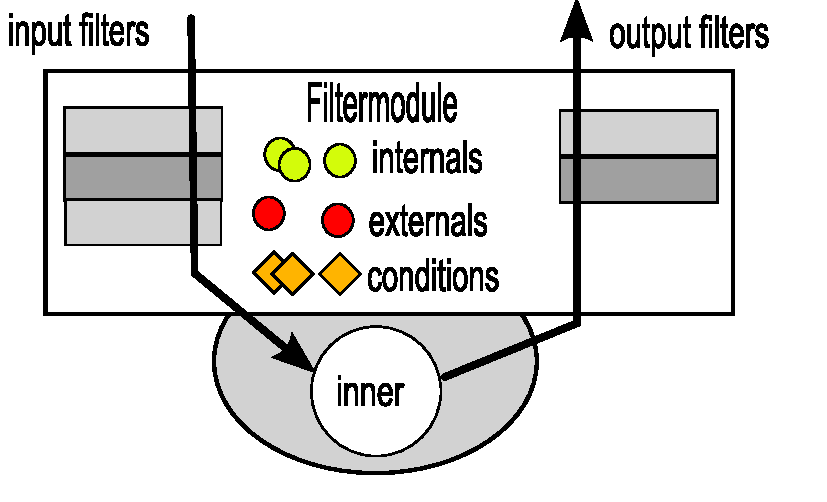
\includegraphics[style= fourthheight]{images/ARM-filtermodule}
	\caption{Schematic representation of a filter module}
	\label{fig::arm::fm:schema}
\end{figure}
A filter module is an entity that holds filter sets which are composed together.
The objects and the conditions that are used in the filters are also declared in the filter module.
\autoref{fig::arm::fm:schema} demonstrates how a filter module can be visualized in a schema.
The schema shows a filter module superimposed to an object, this object is called the ``inner'' object.
Any message that is sent to the object goes through the input filters and any message that is sent goes through the output filters. 
Both filter sets can use internals, externals, and conditions.
These elements are declared in the internals, externals, and conditions blocks.

\section{Examples}
\begin{lstlisting}[caption={Dynamic strategy filter module from Pacman },label=lst::ARM:fil:example1,style=listing,language=ComposeStar,float=[tpb]]
filtermodule dynamicstrategy{
  internals
    stalk_strategy : pacman.Strategies.StalkerStrategy;
    flee_strategy : pacman.Strategies.FleeStrategy;   
  conditions
    pacmanIsEvil : pacman.Pacman.isEvil();
  inputfilters
    stalker_filter : Dispatch = {!pacmanIsEvil => 
      [*.getNextMove] stalk_strategy.getNextMove};
    flee_filter : Dispatch = {[*.getNextMove] flee_strategy.getNextMove}
}
\end{lstlisting}
\begin{lstlisting}[caption={Enqueue filter module from Jukebox },label=lst::ARM:fil:example2,style=listing,language=ComposeStar,float=[tpb]]
filtermodule Enqueue{
  externals
    playlist: Jukebox.Playlist = Jukebox.Playlist.instance();
  inputfilters
    meta : Meta = { True => [*.play] playlist.enqueue}
}
\end{lstlisting}
A filter module can contain parameters, internals, externals, conditions, input filters, and output filters.
The blocks in which these filter elements are declared are all optional, so the shortest filter module you can write is \lstinline!filtermodule fm {}!. 
\autoref{lst::ARM:fil:example1} and \autoref{lst::ARM:fil:example2} show two example filter modules taken from the \Compose* example directory~\cite{Composestar}. 
How the filter module elements work is explained in their respective chapters.
The examples are given to get an idea of how to build up a filter module.
The ordering of the blocks is fixed, therefore it is not possible to place the conditions block before the internals block.

\section{Legality Rules}
\begin{itemize}[noitemsep]
\item The identifier of a filter module must be unique for the concern where it is declared in;
\item The blocks in a filter module must be in the following ordering: internals, externals, conditions, input filters, and output filters;
\item You can only have one declaration of the above mentioned blocks, for example there can be only one set of internals.
\end{itemize}

%\faq{} no questions, should be clear, I'm not going to think any questions and hints
\comments{
\para{Language Independence}
\begin{lstlisting}[caption = {A filter module with a primitive value}, label = lst::ARM:int:example3,
style = listing, language =ComposeStar, float = tpb]
filtermodule rollbackcounter{
  internals
    counter : int;
  inputfilters
    e : Error = {(if counter > 10) => [*.*]};
    m : Meta = {[*.rollback] counter++;}
}  
\end{lstlisting}
\begin{lstlisting}[caption = {A filter module with an object instead of primitive value}, label = lst::ARM:int:example4,
style = listing, language =ComposeStar, float = tpb]
filtermodule rollbackcounter{
  internals
    counter : Counter; // extends of Integer
  conditions
    greaterThenTen : counter.isGreaterThenTen();
  inputfilters
    e : Error = {greaterThenTen => [*.*]};
    m : Append = {[*.rollback] counter.raiseCounter}
}
\end{lstlisting}
It is not possible to use primitive values, like int, char, and bool, as internals and externals,
this is a result from the language independence
we want to have in \Compose*. 
This means that only objects can be used as internals and externals.
Object references are language independent and thus usable in
a language independent environment.
The usage of primitive values in the language
would break language independence because the primitives have different ranges in each 
language\footnote{For bool (or boolean) this is not a real problem, because generally it has only
two values: True and False. However, if we would find (or create) a language that uses fuzzy
values for its booleans then we have the same range problem with booleans as with, for example, integers.
In such scenario the question is whether the fuzzy range is from one to zero or from hundred to zero?}.
There are ideas to introduce a set of primitive values for usage in the filter module,
but these ideas always get stuck on the fact that you need to set a range for the primitives
and they often conflict with the requirement to keep the language as concise as possible.
An example of a rejected solution is the subtyping of integer values like in the programming language Ada~\cite{Ada95}. With Ada it is possible to create a subtype of integer by declaring
it as a subtype of integer and by setting a range, for instance from one to ten.
A possible Ada type declaration is \lstinline|type OwnInteger is Integer range 0 .. 256;|

If we look on how we would put a primitive into action
we can see that we can do the same with an object. For example, if we take a filter module that allows
ten times the call \lstinline!rollback! and gives an error the eleventh time, then the filter module
does need a counter to keep track on how many times the call \lstinline!rollback! has been send to that
filter module. In \autoref{lst::ARM:int:example3} the code with a primitive value is worked out.
In line 3 of \autoref{lst::ARM:int:example3} an integer is declared, we assume that by default the value will be zero. An alternative is to create an internals declaration like
\lstinline!counter : int = 0;!. This value counter is used in line 5 to check whether the amount of rollback is still
below ten. To get the filter module count every call to the method \lstinline!rollback! we need
a statement as \lstinline!counter++! (Line 6). Because the internal is only accessible in the filter module we need
to use a statement in the filter that raises the value of counter.
So with the use of primitive values in the filter module we also need to add operators to use the values.

\autoref{lst::ARM:int:example4} shows the same behavior only with an object that inherits from the
Integer object\footnote{Extending from Integer makes that you can add your own custom methods like \emph{raise()} and
\emph{isGreaterThenTen()}.}.
The internal declaration now uses a Counter class type, the if-statement is replaced with a condition declaration as seen in line 5 and the raising of the counter is now been handled with a function of the class Counter.
This gives that using an object is preferable to a primitive value, because we can use the
methods of the internal and we do not need to introduce mathematical operators, like
``$>$'' and ``$+$'', in the filter syntax. So we can achieve the same with an object or a primitive,
only with the primitive we have problems with breaking language independence and
we have a syntax that is less concise.

Therefore we conclude that we do not need primitive values in the language and we only need method calls
and object references.
Not adding primitive values to the syntax saves us
from the issues mentioned above. First it offers us the possibility to keep the filter module as concise as possible and
second if we would consider adding primitive values and some operators, we would never become as expressive
as the base language, and it is not our goal to copy all the possibilities of the base language.
With this we can close the discussion whether to introduce primitive values in
the filter module.

\para{The Methods Block}
Originally, the filter module also had a method block. As mentioned earlier in ~\cite{Doornenbal2006} it has become obsolete
and it has been removed from the language.

\para{Combining Internals and Externals}
\begin{lstlisting}[caption = {A parameter as external object}, label = lst::ARM:fm:comment1,
style = listing, language =Composestar, float = tpb]
filtermodule agenda(?externalObject){
  externals
    secretary : Example.Secretary = ?externalObject;
}

superimposition{
  filtermodules
    selA <- example(Example.Secretary);
    selB <- example(Example.Secretary);
}
\end{lstlisting}
The internals and externals are the local variables of a filter module. If we look at the example programs in \Compose*, then we see
that the externals are only used in combination with the singleton design pattern~\cite{Gamma95}. Because
the usage of the externals is limited, we can consider combining both blocks into one block called \emph{variables}.
Whether the combination of both blocks is desirable depends whether we want to keep a visible difference
between an internal and external declaration. A solution is to mark externals with a ``*'', like C++ uses for pointers, so that all the
variables are in one field and there is still a (visible) difference between internals and externals.

However, with the introduction of filter module parameters, the usages of the internals and externals fields are extended.
For the externals it means that we can get programs like \autoref{lst::ARM:fm:comment1}. In that example
one instance of the given object is used for all the classes that are bound in the filter module binding, thus
in this particular example there are two instances of the class \lstinline!Example.Secretary!, one for the selection
of classes of selA and of the classes of selB\footnote{The selections can have an overlap.}.
The external declaration on line 3 has an identifier, a fixed type, and a flexible object.
We can apply the ``*'' construction also in this situation, but then you can only derive the meaning of the code with the ``*''. If we would introduce constructor calls for internal declaration we get a readability problem.
Consider the line of code: \lstinline|variable : type = ?parameter;|. If this would be an internal in the
variable block it means that the parameter is cloned, an external in the same variable field is then
\lstinline|*variable : type = ?parameter;|, which means the same as the construct in \autoref{lst::ARM:fm:comment1}.
Due to the new options introduced by the parameters, keeping the distinction between internals and externals becomes
more preferable over the combination of the two blocks.

So with the introduction of parameters, we need to reevaluate the idea of combining the internals and externals fields.
And can conclude that with the
choice of adding parameters to the filter module, it is better to make a clear distinction between externals and internals,
and the best way to do so is to keep them separated.

\para{Block Ordering}
The order of the blocks in the filter module is fixed, making it impossible, for instance, to place externals before internals and to have two conditions blocks. It is
a matter of readability whether mixed ordering and multiple occurrences of blocks are better then fixed ordering and single occurrence of blocks.
Because of the filter operators and how filters work together we only allow one input and output filter set per filter module and that we do not break it up in sub parts. If we would
break up the filter sets, then it becomes harder to read how a filter set behaves.
Another point is that if we would allow the declaration of internals and externals between filters, then users can get confused whether the scope is the whole filter module or just until the next internals or externals block.
Therefore we chose to use the fixed one-of-a-type syntax and that no mixes of blocks are allowed.
}
%\dotnetcomment{
}
%\javacomment{}
%\ccomment{}
%\pending{}
%\furtherreading{}
% empty template for ARM entry. By Dirk Doornenbal. V1.1 17 april 2006
% Filtermodule parameters entry V1.0 22 april 2006
\chapter{Filter Module Parameters}
Filter module parameters can be used to bind variables to a filter module when the filter module is bound to an object.
It is possible to use a single parameter value or a list of parameter values; these will be referred to as \emph{single parameter} and \emph{list of parameters}.
The scope of the filter module parameters is the filter module where they are declared.

\section{Syntax}
Parameters declarations are placed right after the name of the filter module. 
A parameter must have a ``?'' or a ``??'' prefix, followed by an identifier.
The single question mark is for a single value and the double question mark is to mark a parameter list.
After you have declared the parameters you can use them in the filter module. The formal syntax is stated in \autoref{lst::ARM:fmp:syntax}.

\begin{lstlisting}[caption = {Parameter declaration syntax}, label = lst::ARM:fmp:syntax,
style = listing, language = ebnf, float = tpb]
FilterModule ::= `filtermodule' Identifier [FilterModuleParameters] `{'
                  [Internals] [Externals] [Conditions]
                  [InputFilters] [OutputFilters] `}';                                    
FilterModuleParameters ::= `(' ParameterDefinition {',' ParameterDefinition} `)';
ParameterDefinition ::= Parameter | ParameterList;
Parameter ::= `?' Identifier;
ParameterList ::= `??' Identifier;
\end{lstlisting}

You can use a single parameter to parameterize the following elements of a filter module:%
\begin{itemize}[noitemsep]
\item Internal type
\item External type
\item External initialization
\item Condition declaration
\item Filter type
\item Filter arguments
\item Target
\item Selector
\end{itemize}

Lists of parameters can only be used in the selector of a matching.

\section{Semantics}
The parameters are variables that can be used in the scope of a filter module. 
The values of the parameters are assigned with the filter module binding.
Parameter types are inferred automatically; the declaration of a parameter is only the identifier of the parameter with a prefix.

\section{Examples}
The first example, \autoref{lst::ARM:fmp:example1}, shows a filter module that handles logging. 
Logging is a common concern and it is likely that a filter module like this will end up in a concern library. 
The given arguments, in line 1 of the example, are an external declaration, which can be an object or a method that will return an object, a method reference, which must refer to a method that returns a boolean value, and a set of selectors.
The external and condition declaration are like an ordinary declaration only the right hand side of the declaration has now a parameter, thus this part is known when the filter module is bound to an object.
In the filter \lstinline!??setOfSelectors! is used as argument for the selector part, it means that every item of the list will be evaluated, in this example this means that there will be a name matching for the functions \lstinline!print! and \lstinline!printAll!, which are given in the filter module binding in line 12.
In that binding the other two arguments are given as well.

\begin{lstlisting}[caption={Example of a filter module for logging},label=lst::ARM:fmp:example1,
style=listing,language=ComposeStar,float=tpb]
filtermodule logging(?externalDeclaration, ?methodreference, ??setOfSelectors){
  externals
    logger : Logger = ?externalDeclaration;
  conditions
    c : ?methodreference;
  inputfilters
    m : Meta = {c => [*.??setOfSelectors] logger.log}
} 

superimposition
  filtermodules
    self <- logging(Logger.instance(), inner.isActive(), {print, printAll});
\end{lstlisting}

The second example, \autoref{lst::ARM:fmp:example2}, is a generic single inheritance filter module.
The internal declaration is like an internal declaration with a parameter and with the filter module binding a proper class type must be provided. 
The filter in line 5 first uses a signature matching on inner to have the possibility of overriding methods.
 \autoref{lst::ARM:fmp:example3} demonstrates a generic encryption filter module with a parameterized filter type and a parameter list for the selector of the matching part.

\begin{lstlisting}[caption={Example of a generic inheritance filter module}, label = lst::ARM:fmp:example2,
style = listing, language=ComposeStar, float = tpb]
filtermodule inherit(?internaltype){
  internals
    parent : ?internalType;
  inputfilters
    d : Dispatch = {<inner.*> inner.*, <parent.*> *.*}
} 
\end{lstlisting}

\begin{lstlisting}[caption = {Example of an encryption filter}, label = lst::ARM:fmp:example3,
style = listing, language =ComposeStar, float = tpb]
filtermodule encryption(??setOfSelectors, ?filtertype){
  outputfilters
    e : ?filtertype = {[*.??setOfSelectors]}
} 
\end{lstlisting}

\section{Legality rules}
\begin{itemize}[noitemsep]
\item The identifiers of the parameters must be unique for one filter module, so declaring both \lstinline!?para!
and \lstinline!??para! is not allowed. 
So an identifier cannot occur in one filter module with different prefixes;
\item Although you do not need to specify types, there is a typing system for the parameters. 
If there is a typing error the compiler will let you know, for more information on the technical details consult
the implementation details in~\cite{Doornenbal2006};
\item When a filter module defines parameters, the same amount of parameters must be provided in the superimposition.
\item A list of parameters can only be used in the selector of a matching part.
\end{itemize}

\faq{
\para{FAQ}
\question {Because ?parameter is a single parameter and ??parameter a list of parameters, does that mean
that ???parameter is a list of parameter lists?}
\answer{No, because all ``???(?)\mult'' prefixes are too complex to use and during the design of the filter module parameters no general usage could be found for ???parameter.}

\question{How can you determine the types, for example an internal type or a selector, that you need to fill in the filter module binding?}
\answer{You must derive the type information from the filter module specification.}

\para{Hints}
%%michielh: does not belong here?
%The given arguments for the parameters can be a string or a reference to an object.
%Compose* handles the type conversions for string to object reference and vice versa, but when a wrongly typed argument is provided, Compose* will give an error.

In \autoref{lst::ARM:fmp:example1}, line 3, the type of the external is fixed and the initialization expression is made generic with a parameter. 
This construction is more robust than the construction where the type of the external is a parameter as well.
Because with a static type we know that initialization expression must give back the static type, or a type that inherits from the static type.
So if the external declaration is type sound then we also know a part of the signature. 
If we take \autoref{lst::ARM:fmp:example1}, we see that we can write a reusable logging filter module.
The user that reuses this filter module must provide an object with a certain signature.
In this case we want to have at least the method \lstinline !log! in the signature. 
With an external with a generic type it is not possible to enforce this.
}

\comments{
The prefixes are inspired by Sally~\cite{Sally} and LogicAJ~\cite{Logicaj}, which both extend AspectJ with parameters. 
They make the distinction between a single parameter and a parameter list with the different prefixes ``?'' and ``??''. 
When we were looking to parameters we wanted a way to make them distinct from literals, so adding a prefix is
an obvious solution for this.

\para{Typing}
Typing is left out of the grammar because we infer types automatically in Compose*.
This means that the user does not have to define the type, which lowers the complexity of the syntax. 
If there is a problem with incompatible types or parameters used on two places and those places do require
different types, then \Compose* will give an error. 

\para{Not implemented warning}
Filter module parameters are currently only implemented for selectors.
An error will be given when parameters are used in any of the other specified locations.
}

%\pending{}

\furtherreading{
The filter module parameters are introduced in \cite{Doornenbal2006}, here you can find more information on how the syntax was formed and what the other alternatives were.
}
% empty template for ARM entry. By Dirk Doornenbal. V1.2 18 april 2006
% Internals entry V1.0 ?? april 2006
\nomenclature{LHS}{Left Hand Side}%
\nomenclature{RHS}{Right Hand Side}%
\nomenclature{EBNF}{Extended Backus-Naur Form}%
\nomenclature{OO}{Object Oriented}%
\chapter{Internals}%\label{insert_label}
Internals are the object instances that are instantiated for each instance of a filter module. 
Because of this, internals can be used in situations where each instance of a filter module must have its own instance of an object, for example to hold a state or for inheritance by delegation.

\section{Syntax}
The internal declaration has two parts, which are separated with a colon. 
The left hand side contains the identifiers of the internals, and the right hand side the type of those identifiers. 
The formal syntax is defined in \autoref{lst::ARM:int:syntax}.

The types are defined by fully qualified names.
You can refer to an internal in the conditions field, the filter parameters, and the Target.
Internals can only be objects, primitive types are not allowed.
\begin{lstlisting}[caption = {Internals syntax}, label = lst::ARM:int:syntax,
style = listing, language = ebnf, float = tpb]
FilterModule ::= `filtermodule' Identifier 
                  [FilterModuleParameters] `{'
                  [Internals] [Externals] [Conditions]
                  [InputFilters] [OutputFilters] `}';
Internals ::= `internals' {Internal ';'};
Internal ::= Identifier {',' Identifier} ':' Type;
\end{lstlisting}

\section{Semantics}
When the filter module gets instantiated, all its internals get instantiated using the default constructor.
\autoref{lst::ARM:int:example2} shows the binding of a filter module \emph{isActive} to classes A and B. 
The result of this is shown in \autoref{fig::arm::int:initialisation}.
Every instance of A and B gets its own instance of the filter module \emph{isActive} and each instance of the filter module gets its own instance of the internal \lstinline!state!.

The effect is that every instance of an object gets its own instance of the filter module and thus indirect the internal, making it suitable for storing states independently and for inheritance by delegation. 
With the proper filter construction, like \lstinline!d : Dispatch = { <internal.*> internal.*}!, it is possible to extend the signature of a superimposed object with the signature of the internal.
This means that you do not need to access the internal from outside the filter module, because you can directly
use the object on which is superimposed.

\begin{lstlisting}[caption = {Example 2, a filter module to hold a state}, label = lst::ARM:int:example2,
style=listing, language=ComposeStar, float = tpb]
filtermodule isActive{
  internals
    state : State;
  conditions
    notActive : state.notActive();
  inputfilters
    d : Dispatch ={<state.*> state.*};
    e : Error (state) = {notActive => [*.*]}
}
superimposition{
  selectors
    sel = {C | isClassWithNameInList(C,[`A', `B'])};
  filtermodules
    sel <- isActive;
}
\end{lstlisting}

\begin{figure}[tpb]
	\centering
	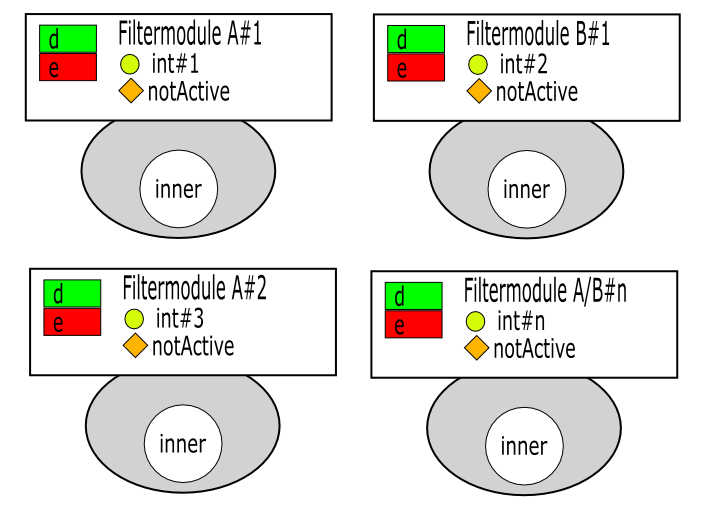
\includegraphics[style=thirdheight]{images/ARM-internalInitialization}
	\caption{Instances of \autoref{lst::ARM:int:example2}}
	\label{fig::arm::int:initialisation}
\end{figure}

\section{Examples}
In the Pacman example (\autoref{lst::ARM:int:example1}), the strategies are internals; this gives that they are instantiated for each filter module. 
An internal is declared with a fully qualified name of a class.

\begin{lstlisting}[caption = {Example 1, a piece of Pacman}, label = lst::ARM:int:example1,
style=listing, language =ComposeStar, float = tpb]
filtermodule dynamicstrategy{
  internals
    stalk_strategy : pacman.Strategies.StalkerStrategy;
    flee_strategy : pacman.Strategies.FleeStrategy;   
  conditions
    ...
\end{lstlisting}

\section{Legality Rules}
\begin{itemize}[noitemsep]
\item The identifier of an internal must be unique for the filter module where it is declared in;
\item The type must be a fully qualified name of a class and this class must exist;
\item In order to be instantiated, the class for the internal must have a public constructor without parameters;
\item When an internal is declared but not used you get a warning from the compiler.
\end{itemize}

\faq{
\para{FAQ}
\question {What is the use of declaring multiple instances of one type? Is it not possible to rewrite the class of the type, so that you only need to declare one internal?}
\answer {This depends on the situation, whereas for holding a state you can also write another class that takes care of the complete state, however for constructions where you delegate to a tree-like structure, like \lstinline!left, right : Node;!, you do not want to combine the internals into one class.}

\question {Is it possible to access an internal of another filter module?}
\answer {It is not possible, on conceptual and implementation level, to access an internal with a filter module element reference.}

\question {I want to declare an internal with a type that is in a library, but the class does not have a default constructor. 
How can I solve this?}
\answer{
The best way to solve this is by extending the class you want to use with a default constructor that sets the needed default values. 
If that is not possible because the class has been made final, then you can write a static method which calls a constructor with arguments and returns the result, this static method can be used in the declaration of an external\footnote{\nb: Only use this construction if you are stuck in such particular situation, see also the commentary.}.
}
 
\para{Hints}
The instantiation of an internal happens with a constructor with no parameters. 
In most object-oriented languages this is the default constructor, which is used when the user does not create a constructor. 
Sometimes people forget to create a constructor without parameters, when there is already a constructor with parameters, which results in an error.
}

\comments{\para{The use of Arguments in Constructors Calls}
The internal initialization is done with a constructor without arguments; this is a result of the requirement to be language independent. 
The internal declaration \lstinline!internal: Person = Person(``Albert'', 24, true);! is considered as language dependent and therefore only constructors without arguments are used. 
We will not re-discuss the point of allowing primitive values in the internal declaration, because is has been discussed in \autoref{chapter:filtermodule}.
However, with the introduction of the filter module parameters it is possible to use objects, which are passed through the filter module parameters, in the declaration of the internals.
This feature is not added to the syntax yet, because it relies on the full implementation of the filter module parameters. 
When this is realized then the syntax can change to the one given in \autoref{lst::ARM:int:syntax2}.
\\\\
\begin{lstlisting}[caption = {Proposed internal syntax}, label = lst::ARM:int:syntax2,
style = listing, language = ebnf]
Internal ::= Identifier {',' Identifier} ':' Type 
              [`=' Fqn `(' FilterModuleParameters `)']
\end{lstlisting}
Because we already use default constructors, we already have the mapping from the language independent declaration to language specific constructor calls, thus we do not have to work them out for adding arguments in a constructor.

\para{Visibility of Internals}
As mentioned in the semantics, it is possible to extend the signature of the class on which is superimposed with the signature of the internal. 
What is not mentioned in the text, is whether the internal is public or private value, and even more important can we directly access the internal?
To start with the public or private matter, addressing the filter module directly from outside the filter module is not correct programming for Compose*, because it breaks with the filter interface. 
So whether it is public or private, you should not access it anyway.

\para{Internals as Externals}
As mentioned earlier in \autoref{chapter:filtermodule} it is good to keep a difference between internals and externals.
It is however, possible to write all internals as externals, if you write a static method \lstinline! static public getnewPerson() \{ return new Person() \} ! and you use that in an external declaration, \lstinline!externals person : Person = person.getNewPerson()!, then you get the same result as when you would create an internal with \lstinline !internals person : Person!.
The construction showed here is not what we want, because we break the decoupling of the main code and the concerns, the class Person, which is in the main code, does have a method which is solely written for a concern.
The only correct use for this construction is when you want to use an internal of a class out of a library, and this class does not have a default constructor and the class is declared as final\footnote{It is actually your only option when you are stuck with such a library.}. 
It is for the best to avoid this kind of constructions; however it is good to know that there are workarounds for this kind of situations.}

\dotnetcomment{If you really want to access an internal then there are two options, first you can access the filter information from the repository, which has at runtime the reference to the internal you want. 
%\footnote{As you might guessed this is actually a hack.}.
Second, it is possible to write a filter that returns the internal and with the extension of the signature of the superimposed object you can get a \emph{get-method} for the internal, this construction is demonstrated in \autoref{lst::ARM:fmp:commentdotnet1}. 
The second option is preferable above the first one, because it is more clear of what you do, only in certain cases where you cannot extend the signature you are stuck with the first option.

\begin{lstlisting}[caption = {How to get hold of an internal}, label = lst::ARM:fmp:commentdotnet1,
style = listing, language=ComposeStar, float = tpb]
filtermodule returnInternal{
  internals
    state : State;
  inputfilters
    d : Dispatch = {[*.getState] s.getSelf}
}
\end{lstlisting}}

%\ccomment{To be specified\\\\\\\\\\}

%\pending{}

%\furtherreading{}


% empty template for ARM entry. By Dirk Doornenbal. V1.5 2 mei 2006
\nomenclature{fqn}{Fully Qualified Name}
\chapter{Externals}
Externals are objects that are instantiated outside a filter module.
They can be instances which are used in multiple places in the application, for instance as a Logger object, or they are shared between multiple filter module instances.

\section{Syntax}
\begin{lstlisting}[caption = {Externals syntax}, label = lst::ARM:ext:syntax,
style = listing, language = ebnf, float = tpb]
FilterModule = 'filtermodule' FilterModuleName [FilterModuleParameters] '{' [Internals] [Externals] [Conditions] [InputFilters] [OutputFilters] '}';
Externals = 'externals' {Identifier ':' Type ['=' InitialisationExpression] ';'};
InitialisationExpression = Fqn '(' [ArgumentList] ')';
ArgumentList = IdentifierOrFMParam {',' IdentifierOrFMParam};
IdentifierOrParameter = Identifier | Parameter;
\end{lstlisting}
As we can see in \autoref{lst::ARM:ext:syntax}, we can split up the external in three parts: the identifier, type, and the optional initialization expression.
The initialization expression is the method that returns the reference to the external object.
It is possible to use arguments in the initialization expression.
Without an initialization expression the external will refer to a static object.

\section{Semantics}
\begin{figure}[tpb]
	\centering
	\includegraphics[style=thirdheight]{ARM-externalInitialization}
	\caption{Schema of \autoref{lst::arm::ext:example1}}
	\label{fig::arm::ext:schema2}
\end{figure}
If we take \autoref{lst::arm::ext:example1} and look how the instances are created, we get \autoref{fig::arm::ext:schema2}.
Every instance of the filter module \lstinline!dynamicscoring! gets a reference to the common object Score.
If we draw a schema of \autoref{lst::ARM:ext:example2} then we get a different picture, because every instance of \emph{delegatePlanning} gets a pointer to one of the two shared externals.

Getting a shared object can be done on several ways, however you must write a construct that holds the objects so that you can select them, thus you should keep a collection of externals. 
If there is only one instance of an external, then the \emph{Singleton} pattern is a good pattern to apply.

\section{Examples}
\begin{lstlisting}[caption = {Dynamic scoring filter module from the Pacman example}, label = lst::arm::ext:example1,
style = listing, language = ComposeStar, float=tpb]
filtermodule dynamicscoring{
  externals
    score : pacman.Score = pacman.Score.instance();
  inputfilters 
    score_filter  : Meta = { [*.eatFood] score.eatFood, [*.eatGhost] score.eatGhost, 
			[*.eatVitamin] score.eatVitamin, [*.gameInit] score.initScore,
			[*.setForeground] score.setupLabel }
}

superimposition{
  selectors
		scoring = { C | isClassWithNameInList
		            (C, ['pacman.World', 'pacman.Game', 'pacman.Main']) };
  filtermodules
    scoring <- dynamicscoring;
}
\end{lstlisting}
\begin{lstlisting}[caption = {An external without the singleton construction}, label = lst::ARM:ext:example2,
style = listing, language = ComposeStar, float = tpb]
filtermodule delegatePlanning(?external){
  externals
    e : Secretary = ?external;
  inputfilters
    d : Dispatch = {<inner.*> *.*, <e.*> e.*};
}

superimposition{
  ...
  filtermodules
    selA <- delegatePlanning(Secretary());
    selB <- delegatePlanning(Secretary());
}
\end{lstlisting}
In the Pacman example, the filter module \lstinline!dynamicscoring! uses an external to keep track of the score (\autoref{lst::arm::ext:example1}). 
For this concern it means that every instance of the classes \lstinline!pacman.World!, \lstinline!pacman.Game!,
and \lstinline!pacman.Main! gets its own instance of the filter module \emph{dynamicscoring} and each of the instances of \emph{dynamicscoring} has a reference to the same instance of \lstinline!pacman.Score!. 
The construction with scoring in Pacman is known as the Singleton pattern \cite{Gamma95}. 
It is also possible to get constructions without the Singleton pattern as demonstrated in \autoref{lst::ARM:ext:example2}, where an object is used as parameter and is assigned through the filter module binding.

\section{Legality rules}
\begin{itemize}[noitemsep]
\item The identifier of an external must be unique for the filter module where it is declared in;
\item The type must be a fully qualified name of a class and this class must exist;
\item The initialization expression must point to a valid method, this often means that you use a static method.
\item Without an initialization expression the external will be a reference to a static object rather than an instance.
\end{itemize}

\faq{\para{FAQ}
\question{How do I create an external that is unique for a certain number of filter module instances?}
\answer{If you want to use an external that is not shared with every instance of the filter module, you can use the filter module parameters to define the different instances for the external.}}
\comments{The advantage of using the Singleton pattern becomes visible when we would use a
parameter as initialization String. In the given example \autoref{lst::arm::ext:example1},
we see that we can address the same instance of Score from three filter modules and that there will only be one
instance of Score in the application. We could do the same without a filter module, by just
adding the Score object to every class. The advantage of the filter is that when we would write
\lstinline[breaklines=false]!score : pacman.Score = ?instance;!, then we only need to change the initialization String
in one spot instead of all the classes where we want to access Score.

\para{The Alternative to Singletons}
With the addition of filter module parameters it is also possible to use a given object from the parameters as an
external. This fixes the old limitation that you had to choose between a singleton construction, which results in that
every filter module points the same object, or to use an internal, which results in that very instance has it own instance of the
internal. In \autoref{lst::ARM:ext:example2} we have an example were two selections, selA and selB, get a different 
instance of the class secretary. Using an object as a filter module parameter makes it possible to use an instance for
a certain selection of filter module instances instead of all filter module instances.

\para{Arguments in the Method Calls}
Currently it is only possible to use the Singleton design pattern for an external declaration. 
This construct is mentioned earlier in~\cite{Doornenbal2006}
for arguments in conditions calls.

\para{Introducing Static Methods}
In the old syntax it was possible to declare an external without an initialization expression. So the syntax was:
\begin{lstlisting}[style=listingWithNoNumbers,language=ebnf]
Externals ::= `externals' (Identifier `:' Type 
              [`=' InitialisationExpression `(' [ ArgumentList ] `)'] `;')*            
\end{lstlisting}

The purpose of such construct is that with an external declaration without an initialization expression it is possible to introduce static methods. A static method from a class can be used without having instantiated an object from this class.
Because the target needs to be an internal, external, or the keyword ``inner'', the only way you are able to substitute the target, so that it is send to a static method, is by declaring the class as an external.
However, this construct has been removed because the construct probably was not placed in the syntax to support the usage of static methods and that it is just an error in the grammar. The theory mentioned above is a possible explanation what the old syntax could mean.}
%\dotnetcomment{}
%\javacomment{}
%\ccomment{}
\pending{Which are declared first, the internals or the externals? 
To be more concrete, will \autoref{lst::ARM:fmp:pending1} work or not? 
And does it always work? 
If the internals are earlier declared then the external, then the example works and there are no further problems. 
(The given example is probably not the best way to combine internals and externals.)

\begin{lstlisting}[caption = {A filtermodule with an external from an internal},label=lst::ARM:fmp:pending1,style=listing,language=ComposeStar,float=tpb]
filtermodule pending(){
  internals
    i : Distribution;
  externals
    e : Object = i.getSingleton();
}
\end{lstlisting}}
%\furtherreading{}
% ARM entry for the conditions.
\chapter{Conditions} \label{ch::arm:con}
The conditions are used to introduce (boolean) methods  in a filter module so that these methods can be used in a filter specification
to influence the behavior of a filter at runtime. To keep the filter specification simple and to reuse declarations, all the conditions of a filter module are declared in one place: the conditions declaration block.
The methods for implementing the conditions can be defined in the inner object (the class where the filter module is superimposed to), internals, externals, or are static methods.

\section*{Syntax}
\begin{lstlisting}[caption={Conditions syntax},label=lst::ARM:con:syntax,style=listing,language=ebnf,float=[tpb]]
FilterModule ::= `filtermodule' FilterModuleName [FilterModuleParameters] `{'
                  [Internals] [Externals] [Conditions]
                  [InputFilters] [OutputFilters] `}'
Conditions ::= `conditions' (Identifier `:' MethodReference `;')*
MethodReference ::= (FilterModuleElement``.''MethodName | FullyQualifiedName)
                    `(' `)'
\end{lstlisting}
From the syntax, \autoref{lst::ARM:con:syntax}, we see that the condition name and declaration are a one-to-one relation. Each condition name must be unique for each filter module and the name may also not be used for an internal or external. There are two forms of declaration: a condition can be declared from
an internal, external, or the inner object and the other option is to use a fully qualified name of a static method.

\section*{Semantics}
A condition declaration labels a method reference with a identifier so that you can use this identifier in the filter specification, instead of a method reference. The method reference of the condition declaration needs to point to a method that returns a boolean.

\section*{Examples}
\begin{lstlisting}[caption={Some condition declarations combined},label=lst::ARM:con:example1,style=listing,language=ComposeStar,float=[tpb]]
filtermodule someConditions{
  internals
    a : VenusFlyTrapExample.Animal;
  externals
    jbframe : JukeboxFrame.JBFrame = JukeboxFrame.JBFrame.instance();
  conditions
    isfly : a.hasPrey(); // Venusfly trap
    isStateChanged : jbframe.isStateChanged(); //Jukebox
    pacmanIsEvil : pacman.Pacman.isEvil(); //Pacman
    isFrame : Composestar.Patterns.ChainOfResponsibility.Click.isFrame();
    // Command of responsibility pattern
    isBlue : inner.isBlue();
\end{lstlisting}
In \autoref{lst::ARM:con:example1} five examples of condition declarations are given. Four of these declarations come from the \Compose* examples~\cite{Composestar}, for each of them is noted in the listing from which example they come. 
The first one shows the usage of an internal, the second one shows the usage of an external.
The third and fourth examples show the use of static methods.
The last example does not come from the example directory, there is a design technical issue why this option is not much used.
There is no example that uses all the different condition declarations in one condition declaration block.

\section*{Legality rules}
\begin{itemize}[noitemsep]
\item The identifier of a condition must be unique for the filter module it is declared in;
\item The condition implementation method that you reference to must exist and it must return a boolean value;
\item A condition implementation method must not have any side effects in the application.
\end{itemize}

%\faq{
%\para{FAQ}
%\question{}
%\answer{}
%\para{Hints}
%} clear chapter no faq according to me...

\comments{\para{Parenthesis and Arguments}
The current implementation does not allow the usage of arguments in the condition declaration.
As mentioned in~\cite{Doornenbal2006}
it is a possible addition to the language to add arguments in the condition declaration, because of the introduction of the filter module parameters.

\para{The Use of Conditions from the Inner Object}
One of the possibilities to declare a condition is to use a boolean method of the inner object. 
As mentioned earlier, this option is not used in the current set of examples. 
We can say that it is not widely used due to two limitations:
the methods must exist and you should know this when you write the selector. 
Filter modules are imposed on multiple classes and when a method of the inner class is used, then all the multiple classes must contain this method.

There are three ways to use a condition from an inner object without getting any problems with non-existing methods. 
The first is to write filter modules for just one class or its child classes. 
The second use for conditions from the inner object is if you select all the classes which implement a certain interface. 
In that scenario you know whether the boolean method is available if it is in the signature of the interface.
The third one is code conventions, if you use a code convention that classes with a certain annotation all have a method called \emph{foo}, then it is also possible to use the conditions from the inner object safely.

\para{Conditions bound to Static Methods}
It is currently not possible to bind conditions to static methods, this functionality has not be implemented.

\para{Language Independent Conditions}
The selector in the superimposition uses predicate queries to select certain attributes of an application. 
It uses a language independent model of language constructs and each language gets translated to this independent model~\cite{Havinga2005}. 
For instance it uses the term namespace, which gets translated to package for the Java language. 
In theory it is possible to write such language independent model on objects and its attributes, so that we can write language independent conditions with predicate queries. 
This would make it possible to write conditions that are reusable even for another platform.}
%\dotnetcomment{}
%\javacomment{}
%\ccomment{}
%\pending{}
%\furtherreading{}
% ARM entry -> Filter
\chapter{Filters} \label{chapter:filter}
Filters are the main part of a filter module, a filter module can have input filters and output filters.
Both the input filters and output filters have the same syntax and therefore we handle them both in this chapter.

A filter has five parts: the filter identifier, the filter type, the condition part, the matching part, and the substitution part. These parts are shown below:

\begin{center}
$\overbrace{stalker\_filter}^{identifier}~:~\overbrace{Dispatch}^{filter~type}~=~\{~\overbrace{!pacmanIsEvil}^{condition~part} 

\overbrace{=>}^{matching~operator}~\overbrace{[*.getNextMove]}^{matching~part}~\overbrace{stalk\_strategy.getNextMove}^{substitution~part}~\}$
\end{center}

Except for the filter identifier they all are separately described in the reference manual. 
In this chapter we look to how these parts work together and how sequential filters behave.

\section{Syntax} %\label{insert_label}
\begin{lstlisting}[caption = {Filter syntax}, label = lst::ARM:fil:syntax,
style = listing, language = ebnf, float = tpb]

FilterModule = 'filtermodule' Identifier [FilterModuleParameters] '{' [Internals] [Externals] [Conditions] [InputFilters] [OutputFilters] '}';
InputFilters = 'inputfilters' FilterSet;
OutputFilters = 'outputfilters' FilterSet;

FilterSet = Filter {FilterOperator Filter};
FilterOperator = ';';
Filter = Identifier ':' FilterType ['(' [ArgumentList] ')'] '=' '{' FilterElements '}';
FilterType = Identifier;
FilterElements = FilterElement {FilterElementOperator FilterElement};
FilterElementOperator = ',';

FilterElement = [ConditionExpression MatchingOperator] MatchingPatternSet;

ConditionExpression = AndExpression ['|' ConditionExpression];
AndExpression = UnaryExpression ['&' AndExpression];
UnaryExpression = ['!'] ( Operand | '(' ConditionExpression ')' );
Operand = Identifier | 'True' | 'False';

MatchingOperator = '=>' | '~>';
MatchingPatternSet = MatchingPart [SubstitutionPart];
MatchingPart = '{' MatchingPattern {',' MatchingPattern} '}' | MatchingPattern;
MatchingPattern = '[' TargetSelector ']' | '<' TargetSelector '>';
SubstitutionPart = TargetSelector;
TargetSelector = [Target '.'] Selector;
Target = '*' |IdentifierOrParameter;
Selector = '*' | IdentifierOrParameter | ParameterList;
\end{lstlisting}

The syntax in \autoref{lst::ARM:fil:syntax} covers the full syntax of the filter, so it also covers the condition, matching, and substitution part.
The filter type contains the type of the filter, this can be a predefined one (currently Dispatch, Meta, Send, or Error) or a custom type.
A filter element contains an optional condition and operator part and a matching pattern set.
The conditional part contains a logical statement, possibly containing logical operators in combination with conditions and boolean values. 
The message pattern contains a name or signature matching and an optional substitution part. 
The filters are separated with a filter operator. 
Currently the only operator is the ``;''.

\section{Semantics}
As mentioned earlier, a filter can consist of five parts. 
The filter identifier can be used to get the corresponding filter, like other filter module elements. 
The filter element is the combination of condition, matching operator, matching, and substitution part.
How the filter element behaves, depends on the filter type. 
If the condition and matching part matches then the substitution part gets executed.

Filters are separated by a ``;'', this operator means that if the filter does not match, the next filter in the filter module will be evaluated. 
After the last superimposed filter module a \emph{default dispatch filter} to the \emph{inner object} is created. 
This means that the last filter that is declared in a filter module is always followed by another filter, be it from the next filter module or it is the default dispatch filter. 
To keep the user from placing another filter operator between these couplings, it is not possible to use the ``;'' after the last filter in a filter module.

Input filters reason about messages going to the object and output filters on the messages that are sent from an object. 

\section{Examples}
\begin{lstlisting}[caption = {Dynamic strategy filter module in Pacman}, label=lst::arm::fil:example1,style = listing, language = ComposeStar,float=[tpb]]
filtermodule dynamicstrategy{
  internals
    stalk_strategy : pacman.Strategies.StalkerStrategy;
    flee_strategy : pacman.Strategies.FleeStrategy;
  conditions
    pacmanIsEvil : pacman.Pacman.isEvil();
  inputfilters
    stalker_filter : Dispatch = {!pacmanIsEvil => 
      [*.getNextMove] stalk_strategy.getNextMove };
    flee_filter : Dispatch = {[*.getNextMove]flee_strategy.getNextMove }
}
\end{lstlisting}

When we look at the dynamic strategy concern of Pacman, \autoref{lst::arm::fil:example1}, we have two filters: stalker filter and flee filter. 
Both filters are of the filter type dispatch, this means that if the condition part and matching part matches, the target and selector gets substituted with the values in the substitution part and the message is then dispatched to the target of the changed message.

The combination of the two filters means that the stalker filter is evaluated first and if it does not match then the next filter is being evaluated, this is the flee filter in this situation.
The matching is based on the condition part, in the example this is the condition whether Pacman is evil, and the matching part, which filters on messages with ``getNextMove'' as selector value.
When a filter matches, the target and selector of the message gets changed with the values of the substitution part. 
What happens with the message then depends on the filter type.
To specify how sequential filters behave there is an filter operator placed between the filters. 
Currently only the ``;'' is used and it means ``if not then''.  
It is not possible to place an operator after the last filter in a filter set.

\begin{lstlisting}[caption = {Custom logging filter module}, label=lst::arm::fil:example2,style = listing, language = ComposeStar,float=[tpb]]
filtermodule logger(??inputMethods, ??outputMethods){
  externals
    logger : Logger = Logger.instance();
  conditions
    isLoggingOn : logger.isOn();
  inputfilters
    inlog : Meta = {isLoggingOn => [*.??inputMethods] logger.log}
  outputfilters
   outlog : Meta = {isLoggingOn => [*.??outputMethods] logger.log}
}
\end{lstlisting}

An example on how you can place input and output filters in one filter module is demonstrated in \autoref{lst::arm::fil:example2}. 
In the example the working of both filters is the same, if the condition matches and the selector is in the set of the given methods, then the message getss wrapped up and is send to the external object and to be more precise to the method \lstinline|log|.

\section{Legality Rules}
\begin{itemize}[noitemsep]
\item The identifier of a filter must be unique for the filter module where it is declared in, so it is not possible to have the same name for an input and output filter;
\item Filters are separated by a ``;'', which is called the composition operator;
\item The last filter is not followed by a ``;''.
\end{itemize}

\faq{
\para{FAQ}
\question{Why is it not possible to place a ``;'' after the last filter?}
\answer{The ``;'' between filters is often mistaken for a terminator symbol, but it actually says something
about the sequential ordering of filters. 
The last filter in a filter module is always followed by the filter of the next filter module or the default dispatch filter. 
It would be incorrect to let the user have a say about that coupling and therefore it is not possible to place a ``;'' after the last filter.}

\para{Hints}
To keep a message from being evaluated by the default dispatch filter it is possible to place a last filter that catches all
messages. 
This could be an error or a dispatch filter.
}
\comments{
\para{Filter Identifier}
The filter has a unique identifier which gives the opportunity to get a filter from its filter module by
using a filter module element reference. Currently this construct is not used in \Compose* and it comes from the original idea to reuse filter specifications.
So at the moment the identifier is redundant, but we keep it in the syntax for usability and user-friendliness. Because talking about the fleeStrategy filter is easier
than talking about the first filter of filter module dynamic strategy.

\para{Filter Modules with both Input and Output Filters}
As mentioned earlier it is possible to have input and output filters in one filter module. However, the option of using both input and output filters in a filter module is barely used.
One of the reasons for this is that for most usages of the filter module you only need one of the two filter sets. Some of the used constructs for filters only need an input filter, like for instance the dynamic strategy filter module in Pacman (\autoref{lst::arm::fil:example1}) or a generic inheritance filter module (\autoref{lst::ARM:fmp:example2}).

\begin{figure}[tpb]
	\centering
	\includegraphics[style=thirdheight]{ARM-filter-constraints}
	\caption{Two filter modules with input and output filters}
	\label{fig::arm::fil:comment1}
\end{figure}

A limitation for having both input and output filters in one filter module is how the constraints are defined. For instance, if we take two filter modules logging and inheritance and they both have input and output filters and we want to log before the input filters of inheritance and we want to log after the output filters of inheritance, this is demonstrated on the left side of \autoref{fig::arm::fil:comment1}. However in reality
you end up with the situation on the right, and the only way to get it like the left image is when you break up one of the two filter modules.
To avoid situations like this, it is advisable to only combine input and output filters if it is really necessary, for instance if they share an internal.

\para{Filters as State Machines}
\begin{lstlisting}[caption = {Idea for a filter state machine}, label=lst::arm::fil:comment1,style = listing, language = ComposeStar,float=[tpb]]
inputfilters
  first : Dispatch = {[*.log]} REPEAT
  second : Dispatch = {[*.print]}
}
\end{lstlisting}
\begin{lstlisting}[caption = {State machine with filter operators}, label=lst::arm::fil:comment2,style = listing, language = ComposeStar,float=[tpb]]
internals
  state = State;
conditions
  ifRaisedState : state.ifRaisedState();
inputfilters
  first : Before = {[*.log] *.raiseSate};
  second : Dispatch = {ifRaisedState => [*.print]}
}
\end{lstlisting}
An idea for the usage of the filter operators is to use them for building a state machine. An example is given in
\autoref{lst::arm::fil:comment1}, in this example we want to let the first filter evaluate and when it matches it moves to the second one until that one matches.
Whereas this looks like a nice idea, but there are drawbacks. First you get
problems with the
syntax and semantics, because you must be able to scope your REPEAT statement and you also need to define
what the commando's mean. Second, designing such filter sets is hard and it is much better to write
such a machine with an internal that keeps the state in combination with conditions that handle the state, like \autoref{lst::arm::fil:comment2}.
The filter of the message for the state change can be done with a meta filter or even the prepend and append filter~\cite{Minnen2006}. Writing such construction is easier then using state machine operators.

\para{Filter Operators and Different Filter Combinations}
The filter operator is placed between filters. At the moment only the ``if not then'' operator is used which is in the ``;'' token in the syntax. There are two points to comment on the filter
operator. The first question is why the usage of ``;''? And the second question is can the filter operator mean anything at all?

To start with the second question, as mentioned above with designing the state machine it hard to define new filter operators because you probably end up adding parenthesis and other syntax constructs. Therefore there is no final answer on this question yet, there are some ideas on more filter operators around. But these ideas have problems on the what the semantics are of these operators.
And to answer the first question, it is indeed a bit strange to use the semicolon as an operator. In most programming languages it marks the end of a statement. We do not allow
a semicolon after the last filter declaration and this often regarded as annoying by the users. We could add the ``+'' sign as a stand in for ``;'' to make things less confusing. We have not done it yet, due to the fact that we cannot answer the second question yet and it would
be strange to start adding operators while we have not answered some of the problems with combining filters.

}
%\dotnetcomment{}
%\javacomment{}
%\ccomment{}
%\pending{}
%\furtherreading{}
\chapter{Filter Type} \label{chapter:filtertype}
The type of a filter specifies how a filter behaves for an accept and a reject of the condition and the matching part.
This includes the specification of how to execute the substitution part.
There are currently four predefined filter types and it is possible to create custom filter types.
It is possible to add arguments in a filter specification, it depends on the filter type what the semantics
are of the arguments.

\section*{Syntax}
\begin{lstlisting}[caption = {Filter type syntax}, label = lst::ARM:filtype:syntax,
style = listing, language = ebnf, float = tpb]
Filter = Identifier ':' FilterType ['(' [ArgumentList] ')'] '=' '{' FilterElements '}';
FilterType = Identifier;
\end{lstlisting}
As demonstrated in \autoref{lst::ARM:filtype:syntax}, a filter type it must be a predefined filter type or custom defined one. It is not possible
to overwrite the predefined filters, so a dispatch filter always behaves the same.

\section{Semantics}
There are a couple of builtin filter types:
\begin{description}[style=nextline,noitemsep]
\item [Dispatch] If the message is accepted, then the target and the selector of the message get substituted with the values of the target and selector of the substitution part. 
If the value is a wildcard (``*''), then theoriginal value remains unchanged. 
After that, the message is dispatched to the target of the message; this can be either the old target or a new one. 
In the situation that the target is the old value, the message starts again at the begin of the input filter set. 
A dispatch to inner goes directly to the inner object. 
Dispatch can only be used for input filters;
\item [Send] The send filter is the dispatch filter for the output filters. 
When the filter matches the target and the selector gets substituted with the values that are in the substitution part;
\item [Error] An error filter raises an exception when it rejects. 
It ignores the substitution part;
\item [Meta] When a meta filters matches it reifies the current message and add it as an argument of a new message.
This new message is sent to the object and method declared in the
substitution part. This method must have a single parameter of the type \emph{ReifiedMessage}. 
In this method it is possible to alter the message and to let it resume or to send it back.
\item[Before] This filter will call the method defined by the substitution part when the current message matches.
After this the next filter will be evaluation, thus this filter type does not change the flow of the message.
\item[After] This filter is similar to the \emph{before} filter, except that it will execute the method when the message returns from execution.
For example an \emph{error} filter could disrupt the behavior of this filter because the error filter prevents the execution of the message this filter matches on.
\end{description}

A custom filter gets extended from a meta filter and it is possible to define how it handles the different parts
and values.

\section{Examples}
\begin{lstlisting}[caption={Some different filter types },label=lst::ARM:ft:example1,style=listing,language=ComposeStar,float=[tpb]]
...
inputfilters
  d : Dispatch = {<inner.*> inner.*};
  rotate : Rot13 = { [*.ReadLine] };
  l : Log (?argument) = {[*.log]};
  e : Error = {[*.*]}
}
\end{lstlisting}
In \autoref{lst::ARM:ft:example1} four different filters are used, the first and last filter declaration use predefined filter types, the other two use custom filter types. 
An example of how to write a custom filter type is demonstrated in the Rot13 example~\cite{Composestar}.
It is possible to initialize a custom filter with the filter parameters.

\section*{Legality Rules}
\begin{itemize}[noitemsep]
\item A custom filter type cannot have the same name as a predefined one;
\item A custom filter type must a have an implementation in the application.
\end{itemize}

%\faq{}
\comments{
It is not possible to redefine predefined filter types, this is done to keep the language understandable for a user because in this way a dispatch filter will always behave like a dispatch filter.

The advantage of predefined filters is that we know what they do and therefore we can do a static analysis on the flow of a filter set. 
With a meta filter we do no longer know what happens, because the resume and return commands of a message are called in the implementation. 
On the other hand, predefined filter types are only a selection of possibilities and the meta filter is a necessary type for creating other non-predefined behavior.
So it is a constant trade-off between being all flexible by only using custom filters or just trying to add predefined or custom defined filters for every situation, just to have filter sets where you can reason about.
Therefore we keep the current set of predefined filter types, however there is room for some more predefined filter types.

\para{Runtime vs Inliner}
Not all filters mentioned previously are available for all ports.
The ports that use the runtime (\Compose*[DotNet] and \Compose*[Java]) do not support the \emph{before} and \emph{after} filters.
However, this functionality can be implemented using a \emph{meta} filter.

The ports that use the inliner (StarLight) do not support the \emph{meta} filter.
The meta filter can be partially simulated using custom filters.

\para{Parameters}
Filter parameters, as shown in \autoref{lst::ARM:ft:example1}, are currently not implemented.
\Compose* will accept its usage, but after that they are ignored.

}
%\dotnetcomment{}
%\javacomment{}
%\ccomment{}
%\pending{}

\furtherreading{
More information about the filter and message behavior can be found in \cite{DeRoo2007} and \cite{Hendriks2007}.
}
% Condition part ARM entry. By Dirk Doornenbal. V1.5 2 mei 2006
\chapter{Condition Part} \label{chapter:conditionpart}
The condition part of a filter contains the conditions and operators which say something of the matching part, to reason whether a filter is accepted or not. 
The used methods must be first declared in the conditions block of a filter module. The logical operators are the basic set of \emph{and}, \emph{or}, and \emph{not} added with
two operators to denote ``if true'' (\lstinline[language=Composestar]|=>|) and ``if false'' (\lstinline[language=Composestar]|~>|)., which are placed in front of the matching part.

\section*{Syntax}
The syntax of the condition part, as demonstrated in \autoref{lst::ARM:cp:syntax}, follows the standard way to
program a set of AND (\lstinline|&|), OR (\lstinline$|$), and NOT(\lstinline|!|) operators. The precedence is that the NOT is executed first, then the AND and the OR. This means
that \emph{A AND B OR C} is actually \emph{(A AND B) OR C}. The chosen precedence is the commonly used one.

\begin{lstlisting}[caption={Filter condition part syntax},label=lst::ARM:cp:syntax,style=listing,language=ebnf,float=tpb]
FilterElement = [ORExpression ConditionOperator] MessagePattern
ORExpression = ANDExpression [`|' ANDExpression]
ANDExpression = NOTExpression [`&' NOTExpression]
NOTExpression = [!] (ConditionLiteral | `('ORExpression`)')
ConditionLiteral = ConditionName | `True'| `False'
ConditionOperator = `=>'| `~>'
\end{lstlisting}

The \emph{ConditionLiteral} can be either a condition name, which must be declared in the condition block of a filter module,
or the predefined conditions ``True'' or ``False''. It does not matter whether the keywords are written like this or without
capitals. If there is an expression then there also must be a \emph{ConditionOperator}, there are two options for this
operator: \lstinline[language=Composestar]|=>| and \lstinline[language=Composestar]|~>|.

\section*{Semantics}
In the condition part it is only possible to use the boolean values \emph{true} and \emph{false} or conditions that are declared in the conditions block of a filter module.
This means that the number of possible syntax constructs is small.
The meaning of the logical operators is the same as the usual meaning in most programming languages. The condition operator
does say something on the message part and not as it might suggest on the condition part. The \lstinline|=>| operator
provides a true if the message part matches. The other operator, \lstinline[language=Composestar]|~>|,
gives a true when the message part does not match.

The condition part is optional; however when it is left out then the syntactic sugar places a \lstinline|True =>|
in the filter.

\section*{Examples}
In the Pacman example of \cite{Composestar} we have already seen the filter demonstrated in \autoref{lst::armcp:example1}. In that example the method \emph{pacmanIsEvil}
is checked in order to determine how the ghosts must behave. So when Pacman is not evil it only depends on the matching part whether the filter matches.

\begin{lstlisting}[caption={The dymanic strategy filtermodule}, label=lst::armcp:example1,style=listing,language=Composestar,float=[tpb]]
conditions
  pacmanIsEvil : pacman.Pacman.isEvil();
inputfilters
  stalker_filter : Dispatch = {!pacmanIsEvil => 
                              [*.getNextMove] stalk_strategy.getNextMove};
  flee_filter : Dispatch = {[*.getNextMove] flee_strategy.getNextMove}
\end{lstlisting}

Some examples of condition parts are given in \autoref{lst::armcp:exampl2}. We see that d1 (on line five) depends on the condition isBlue whether the message will pass.
The \lstinline[language=Composestar]|~>| means exclusion so it will match if the message does not
match with the matching part of the filter. Thus
filter d2 (on line six) will never match, because the matching part will always match.
Filter d3 (on line seven) shows a combination of operators and values.

\begin{lstlisting}[caption={Possible condition parts}, label=lst::armcp:exampl2,style=listing,language=Composestar,float=[tpb]]
conditions
  isBlue : inner,isBlue();
  isMorning : inner.isMorning();
inputfilters
  d1 : Dispatch = {!isBlue => *.*};
  d2 : Dispatch = {isBlue ~> *.*};
  d3 : Dispatch = {(isBlue | isMorning) & True => *.*}
\end{lstlisting}

\section*{Legality rules}
\begin{itemize}[noitemsep]
\item A condition name must be declared in the condition block of the same filter module;
\item The keywords true and false are written as ``True'', ``true'', ``False'', and ``false'', anything else, also with different
capital letters, is considered a condition name.
\end{itemize}

\faq{
\para{Hints}
Whereas the condition part is optional, the matching part is not. It is however easy to let only
a condition part determine the outcome of a filter, with the matching \lstinline|[*.*]| every message matches and it only depends on the conditions whether a message is accepted.
}

\comments{\para{Basic Set of Logical Operators}
The supported set operators are the \emph{and}, \emph{or}, and \emph{not}. These three are enough to create any other possible logic operator because they form a \emph{functional complete} set~\cite{vanBenthem91}.
Because we want to reason about the filters, we keep the syntax as simple as possible on this point. It is easier to write an algorithm that only has to take care of three
operators instead of a whole set.

We could go further by removing all the operators and just write one method that calls all the separate
conditions, however this would also mean that this method should also know the references to the internals, externals,
and inner object, and even more important this method would be quite complex and not be reusable at all. Therefore we adopt a limited set
of logical operators.

%\dotnetcomment{
%As of 0.6 this is properly implemented
%\para{Current Implementation}
%Currently the condition part is not programmed as described in this chapter; the nesting is not in the logical operators yet.
%Thus \lstinline|(True & False) & True| will give an error. Because the \Compose* grammar is the same for all ports it therefore
%affects every port.
%}
}
%\dotnetcomment{}
%\javacomment{}
%\ccomment{}
%\pending{}
%\furtherreading{}
% empty template for ARM entry. By Dirk Doornenbal. V1.5 2 mei 2006
\chapter{Filter Matching Part}
The matching part of a filter is where the message is being matched. There are
two different types of matching: name and signature matching.

\section*{Syntax}
\begin{lstlisting}[caption={Filter matching part syntax},label=lst::ARM:mp:syntax,style = listing,language = ebnf,float=tpb]
FilterElement ::= [ConditionExpression ConditionOperator] MessagePattern
MessagePattern ::= Matching [SubstitutionPart]
                   | MatchPattern
                   | `{' Matching (`,' Matching)* `}' [SubstitutionPart] 
Matching ::= SignatureMatching | NameMatching
SignatureMatching ::= `<' MatchPattern `>'
NameMatching ::= `[' MatchPattern `]' | Quote MatchPattern Quote
MatchPattern ::= [Target `.'] Selector
\end{lstlisting}
The syntax of the matching part is shown in \autoref{lst::ARM:mp:syntax}. The basic form is
\lstinline|target.selector| surrounded by the tokens that mark the type of matching. It is possible
to leave out these tokens when only a single MatchPattern is used, in that situation signature matching is applied by default.
The target needs to be an internal, external, or the keyword \emph{inner}. The selector must be a method name.
To indicate whether you want to use name matching or signature matching you can use square brackets (\lstinline![]!) or double quotes (\lstinline!`` ''!) for name matching and angle brackets (\lstinline!< >!) for signature matching.

\section*{Semantics}
The name matching checks the target part of the match and the
selector part. The use of the keyword ``inner'' 
is, as you might expect, quite trivial for a name matching in an input filter.

Signature matching checks whether the selector of the message is in the signature of the given target. This means that it is only useful to fill in the target when a signature matching is used.
Filling in the selector in the signature matching has no use, because \lstinline|<foo.bar>| will
always hold or always fail.

Both the target and the selector can be a parameter, for the selector it is also possible to use a list of parameters.
With a list of parameters it means that one entry in the list must match.

When you have a dispatch filter ands the selector is not in the signature of the object on which is superimposed, then the selector is added to the
signature of this object. This mechanism is not used when a wild card is used on the selector spot,
because that would imply that the signature becomes every possible method. The mechanism also works on singnature matching, which makes it possible to add the signature of the internal or external to the object on which is superimposed.

\section*{Examples}
Three matching parts are demonstrated in \autoref{lst::ARM:ARMMP:example1} line 3. The first two
are of the \emph{name matching} type and the third is an example of \emph{signature matching}.
The matching \lstinline|[tar.sel]| first whether the target points to the same object as where ``tar'' refers to and
it will try to match whether the selector is ``sel''. The second one,
\lstinline|[*.sel]| ignores the target, because a wild card (``*'') is used and the selector is matched
with ``sel''. The last one, \lstinline|<tar.*>| checks whether the selector is in the signature of ``tar''.

The second filter d2 on line 4 demonstrates how you can do a name matching where the selector must match when the selector is not \lstinline!foo! and not \lstinline!bar!.
The matching works as follows, when a selector is one of the values of the list you get a match. Because of the \lstinline[language=Composestar]|~>| this match becomes a reject, thus making this
filter to reject when the selector is \lstinline!foo! or \lstinline!bar!.
Especially for this type on of constructions a matching list is introduced.

\begin{lstlisting}[caption={Some possible matching parts},label=lst::ARM:ARMMP:example1,
style=listing,language =ComposeStar,float=tpb]
filtermodule example{
  inputfilters
    d : Dispatch = {[tar.sel] *.*, [*.sel] *.*, <tar.*> *.*};
    d2 : Dispatch = {True ~> {[*.foo] , [*.bar]} inner.*}
\end{lstlisting}

It is also possible to use parameters as the target and the selector, for the target
only a single parameter can be used, while for the selector both a single parameter and a list of parameters can be used.

\section*{Legality rules}
\begin{itemize}[noitemsep]
\item The used target must be a declared internal, external, the keyword ``inner'', or a parameter;
\item A selector can be a method, a single parameter, or a list of parameters.
\end{itemize}

\faq{
\para{FAQ}
\question{Why is it not possible to use class names as targets?}
\answer{The messages are sent from object to object, therefore the choice is made to use objects as targets instead
of class names. The used identifier in the filters refers to internals, externals, or is the inner object (the object where is superimposed on).
It is however possible to achieve filtering on class names with a meta filter.
}

\para{Hints}
Keep an eye on the \lstinline|[*.*]| because any declaration afterwards does not get reached at all. Another
important thing is that in order to make exceptions for a \lstinline|[*.*]| matching, you can place a filter before
that matching.
}

\comments{With the new proposed filter layout \cite{Doornenbal2006} it is possible to filter on more then just the target and the selector. 
It is known that the current system is too limited to the users.

\para{Wildcards}
In AspectJ it is possible to define pointcuts with wildcards in the method name, like \lstinline!set*!. 
We are aware that \Compose* is indeed not AspectJ, but the idea of using wildcards is tempting, because it is a quick language construct. 
The disadvantage is that \lstinline!set! is open-ended and that a method like \lstinline!setup! is taken into the selection as well. 
A better solution is to use design documentation, like annotations, instead of a wildcard.
In ~\cite{Nagy2006} a proposal is made to use annotations in the matching part, it is has not been implemented yet and therefore the language changes are not mentioned in this chapter. 
Filtering on annotations is covered by the new filter element syntax, however the syntax is different from the original proposal.

%%michielh: no long true?
%\para{Signatures}
%Despite of its name, signature matching only matches on the names of the methods in a class, instead of
%the whole signature. 
%To check on the whole signature you need a meta filter and you have to write the check function yourself. 
%Also filling in the selector in the signature matching has no use, because \lstinline|<foo.bar>| will always hold or always fail.

\para{Inner, Self, Server, and Sender}
In \cite{bergmans:phd94} there are more predefined keywords that say something about the object, on which is superimposed, than just the keyword \emph{inner}. 
In that plan the keywords \emph{self}, \emph{server}, and \emph{sender} can be used in the matching and substitution part. 
Self is the object on which is superimposed plus the extended signatures, thus the original object plus the filter modules.

The \emph{server} keyword points to the original target and selector of a message, thus the original message before it goes into the set of filter modules. 
\emph{Sender} is the object that sends the message. 
The \emph{server} and \emph{sender} can be retrieved in a meta filter.

With \emph{self} we need to determine whether \emph{self} is the extended object after all filter module bindings or just after some of the filter module bindings. 
With this definition you are never sure how the self object looks like, because the self object is flexible due to the possibility that more filter modules are added to the object. 
So it is better to leave self out of the language.

%\dotnetcomment{
%Whether the mechanism to add the selectors of a name matching to the superimposed object depends on the filter type is still an open question. 
%Practically we can apply the mechanism to all filters, the only conceptual point is whether we should also include it for the error filter. 
%Because this last filter does not add any behavior as in adding methods to a superimposed object, the mechanism must not work for the error filter. 
%In \autoref{chapter:filtertype} there is an overview of which filter type uses the mechanism and which does not.
%}}
%\dotnetcomment{}
%\javacomment{}
%\ccomment{}
%\pending{}
%\furtherreading{}
% empty template for ARM entry. By Dirk Doornenbal. V1.5 2 mei 2006
\chapter{Filter Substitution Part}
The substitution part of a filter is where you can specify the changes in a message. Just like the
matching part it consists of a target and a selector.

\section*{Syntax}
The syntax is almost similar to the matching part and is shown is \autoref{lst::ARM:sp:syntax}. The difference is
that the substitution part does not have any brackets, creating a visible difference between matching and substitution part. Another difference is that it is not possible to have a list of substitution parts.

\begin{lstlisting}[caption={Filter substitution part syntax},label=lst::ARM:sp:syntax,style = listing,language = ebnf,float=tpb]
FilterElement = [ConditionExpression ConditionOperator] MessagePattern
MessagePattern ::= Matching [SubstitutionPart]
                   | MatchPattern
                   | `{' Matching (`,' Matching)* `}' [SubstitutionPart] 
Matching ::= SignatureMatching | NameMatchingSubstitutionPart = [Target `.'] Selector
\end{lstlisting}

\section*{Semantics}
A substitution part gets executed when a filter matches, how it gets executed depends on the filter type.
The meaning of the substitution part is simple, if there is a wild card on the target or selector spot the attribute of the message
stays the same. Otherwise the attribute gets substituted with the given value.

\section*{Examples}
In \autoref{lst::ARM:ARMSP:example1} three out of the four possible substitution part combinations are demonstrated. The matching parts are different as well to get a filter specification that means something.
The fourth is that the target stays the same and that the selector changes.

\begin{lstlisting}[caption={Some possible substitution parts},label=lst::ARM:ARMSP:example1,
style=listing,language =ComposeStar,float=tpb]
filtermodule example{
  inputfilters
    d : Dispatch = {[tar.sel] tar1.*, [*.sel] tar2.sel2, <tar.*> *.*}
\end{lstlisting}

\section*{Legality rules}
\begin{itemize}[noitemsep]
\item The used target must be a declared internal, external, the keyword ``inner'', or a single parameter;
\item A selector can be a method or a single parameter;
\item A selector cannot be a list of parameters.
\end{itemize}

\faq{
\para{FAQ}
\question{Why is it not possible to use a parameter list in the selector of a substitution part, like in the matching part?}
\answer{A message can only be send to one method, so a list of methods would be meaningless.}

\para{Hints}
Keep an eye on where you send your messages to. If the combination of target and selector does not exist you get an error,
but it is easier to find the error before it occurs.
}

\comments{Just as with the matching part we can only work with the target and the selector. 
With the proposed new filter layout (\cite{Doornenbal2006}) we can alter more attributes of a message.

\para{Substitution and the disable operator}
When using the disable operator \lstinline[language=Composestar]|~>| the substitution part must use the wild card for the selector, or otherwise limit the signature space in an earlier filter in the same filter module. 
This restriction is caused by the fact that the disable operator matches on everything except the list given in the matching part. 
This makes the number of signatures that match this filter definition infinite, and therefor the substitution part can not be validated if it maps to a single selector. 

\autoref{lst::ARM:ARMSP:example2} is an example of an invalid definition that results in an infinite signature. 
A method to limit the signature space is shown in \autoref{lst::ARM:ARMSP:example3}. 
The error filter restricts the number of signatures passed to the second filter to only those that are defined in the inner class. All dynamically created signatures will be intercepted by the error filter.

\begin{lstlisting}[caption={Infinite signature definition},label=lst::ARM:ARMSP:example2,
style=listing,language =ComposeStar,float=tpb]
filtermodule example{
  inputfilters
    d : Dispatch = {True ~> [*.foo] inner.bar }
\end{lstlisting}

\begin{lstlisting}[caption={Limiting signature space},label=lst::ARM:ARMSP:example3,
style=listing,language =ComposeStar,float=tpb]
filtermodule example{
  inputfilters
    e : Error = { <inner.*> };
    d : Dispatch = {True ~> [*.foo] inner.bar }
\end{lstlisting}
}

%\dotnetcomment{}
%\javacomment{}
%\ccomment{}
%\pending{}
%\furtherreading{}

\chapter{Superimposition} \label{chapter:superimposition}
The superimposition part of a concern is where you can make a selection of program elements, such as classes, and then superimpose certain entities, such as filter modules and annotations, on this selection.

The superimpositions parts are executed during the initialization of the application, this is necessary because the bindings need to be known before the execution starts.

With the changes in the filter module syntax, the superimposition syntax needs some minor adjustments as well.
The superimposition and its fields are all quite young, and moreover it is possible for all fields to point to the original proposal, were the field is proposed.

The superimposition part with the original selector and filter module binding are introduced by~\cite{salinas:ms01}. 
The new improved selector and annotation binding are introduced by~\cite{Havinga2005}.

\section{Syntax}
\begin{lstlisting}[caption = {Superimposition syntax}, label = lst::ARM:si:syntax, style = listing, language = ebnf, float = tpb]
Superimposition = '{' [Conditionals] [Selectors] [FilterModuleBindings] [AnnotationBindings] [Constraints] '}';
\end{lstlisting}
The syntax, as demonstrated in \autoref{lst::ARM:si:syntax}, shows the syntax of the superimposition part. 
The result is the skeleton as demonstrated in \autoref{lst::ARM:si:example1}.

\section{Semantics}
The superimposition itself is a holder of blocks for selecting elements and defining bindings. 
It is executed during initialization of an application.

\section{Examples}
\begin{lstlisting}[caption={The superimposition skeleton}, label = lst::ARM:si:example1,
style=listing, language =ComposeStar, float = tpb]
superimposition{
	conditions
	  ...
  selectors
    ...
  filtermodules
    ...
  annotations
    ...
  constraints
    ...
}
\end{lstlisting}
A superimposition can have five blocks and the ordering of these blocks are fixed, the skeleton is demonstrated in \autoref{lst::ARM:si:example1}. 
There is also only zero or one instance of a block. 
The selectors makes a selection of language elements, which can be used in the filter module and annotation binding.
The conditions can be used for conditional binding of filter modules, and the constraints can be used to force an order of filter modules.

\section{Legality Rules}
\begin{itemize}[noitemsep]
\item The ordering of the sub blocks is fixed and have the following ordering: conditions, selector, filter modules, annotations, and constraints;
\item Each sub block can only have one instance.
\end{itemize}

%\faq{} -> clear no faq
\comments{
\para{The Ordering of the Selector Parts}
The ordering and number of occurrences of the sub blocks is fixed, this is characteristic for the whole \Compose* syntax.
The main reason to do so, is that this ensures that all the declarations of a certain type are all together placed on the same spot. 
Thus you can find all the selectors within one concern on the selectors block. 
It is possible to allow random and multiple placement of the superimposition and its sub blocks. 
However, the readability would drop because users do not longer know where to expect certain blocks. 
To keep everything organized is also the reason why there is only one superimposition block per concern.

\para{Selection of Program Elements}
Currently the selector is used to select only classes. 
However, with the adding the filter module parameters and some other upcoming research it will be possible to select much more then classes and probably you can also superimpose items to the extended selections. 
Therefore the term \emph{program elements} is used instead of classes.

%\dotnetcomment{}
%\javacomment{}
%\ccomment{}
%\pending{}
\furtherreading{
The initial design of the superimposition can be found in ~\cite{salinas:ms01}. More on the design of the new
selector language and the binding of annotations is stated in~\cite{Havinga2005}.
The ideas on the constraints model can be found in~\cite{Nagy2006}.
For the theory behind the removal of the method and condition binding see~\cite{Doornenbal2006}.
}
% empty template for an ARM chapter.
\chapter{Superimposition Conditions}\label{cha:Superimposition_Conditions}

The superimposition conditions are much like the conditions defined in the filter modules.
Except that they can be used for conditional superimposition of filter modules.
This will allow the binding of filter modules to be depended on a runtime variable.

\section{Syntax}

\begin{lstlisting}[caption={Superimposition Conditions Syntax}, label=lst::ARM:sicond:syntax, style=listing, language=ebnf, float=tpb]
Superimposition = '{' [Conditionals] [Selectors] [FilterModuleBindings] [AnnotationBindings] [Constraints] '}';
Conditionals = 'conditions' {SiCondition ';'};
SiCondition = Identifier ':' Fqn ['(' Arguments ')']
\end{lstlisting}

Just like the conditions defined in a filter module, these conditions consist of a identifier and a method that returns a boolean value.
The condition identifier must be unique within the superimposition block.

\section{Semantics}

Each condition is bound to a method.
The method must be a reference to a static method in a defined class.
The condition can be used in the filter module binding part of the superimposition.
It is not possible to use selector values as class reference.
Selectors are often a set of classes, which makes it unclear which class to use for the method binding.

\section{Examples}

\begin{lstlisting}[caption={Some condition examples}, label = lst::ARM:sicond:example1, style=listing, language =ComposeStar, float = tpb]
conditions
      loggingEnabled : BasicTests.ConditionalSuperImpositionTests.LoggingEnabled;
		  timingEnabled : BasicTests.ConditionalSuperImpositionTests.TimingEnabled;
\end{lstlisting}

\autoref{lst::ARM:sicond:example1} shows two defined conditionals. They both point to a static method in the class \lstinline|BasicTests.ConditionalSuperImpositionTests|.

\section{Legality Rules}
\begin{itemize}[noitemsep]
\item The identifier must be unique within the superimposition block;
\item The method must be a public static method;
\item The static method must return a boolean value.
\end{itemize}

%\faq{}

\comments{
\para{Method arguments}
The method arguments are not supported and implemented.
It is currently unclear what values could be passed to these static methods.
It might be a option to use the values of the concern parameters as explained in \autoref{chapter:concern}.

\para{Port support}
Superimposition conditionals are currently only supported in StarLight. 
The runtime ports (\Compose*[DotNet] and \Compose*[Java]) do not support the usage of conditionals.
They will accept it in the language, but they are disregarded in the execution.
}
%\dotnetcomment{}
%\javacomment{}
%\ccomment{}

%\pending{}

%\furtherreading{}

% ARM entry for selector.
\chapter{Selectors} \label{chapter:selector}
The selector field is where you can make a selection of certain program elements. The selections
can be used to bind filter modules or annotations, and it is possible to use the selection as an argument for a filter module parameter.

\section{Syntax} %\label{insert_label}
\begin{lstlisting}[caption = {Selector syntax}, label = lst::ARM:sel:syntax, style = listing, language = ebnf, float = tpb]
Superimposition = '{' [Conditionals] [Selectors] [FilterModuleBindings] [AnnotationBindings] [Constraints] '}';
Selectors = 'selectors' { Identifier '=' '{' ( LegacyExpr | PredicateExpr) '}' ';' };
LegacyExpr = '*' ( ':' | '=' ) Fqn;
PredicateExpr = Identifier '|' ? prolog expression ?;
\end{lstlisting}

The identifier of a selector must be unique for the superimposition where you declare it in. 
There are two available selector expressions: the legacy expression (usage discouraged) and the predicate expression.

The legacy expression always starts with a \lstinline|*| followed by an operator and the fully qualified name of a class.
The \lstinline|=| selects the specified class, and \lstinline|:| selects the specified class and all its subclasses.

The predicate selector consists of two parts, the first part is the identifier that will contain the result of the evaluated predicate expression. 
The second part contains the predicate expression, which is a prolog expression.
This expression should create a result with the identifier specified in the first part.
The list of possible predicate expressions can be found in \autoref{appendix:selectorfunctions}.

\section{Semantics}
With the declaration of a selector you make a selection of program elements and you label these with an identifier.
This identifier can be used in the different bindings and as filter module argument. 
There is a default selector ``self'' which selects a class with the same name as the concern.

\section{Examples}
\begin{lstlisting}[caption={Some selector examples}, label = lst::ARM:sel:example1, style=listing, language =ComposeStar, float = tpb]
selectors
  strategy = 
    { Random | isClassWithName(Random, 'pacman.Strategies.RandomStrategy') };
  levels = 
    { C | isClassWithNameInList (C, ['pacman.World', 'pacman.Pacman']) };
  player = 
    { C | methodHasAnnotationWithName (M, 'Jukebox.StateChange'), classHasMethod(C, M)};
\end{lstlisting}
In \autoref{lst::ARM:sel:example1} there are three example selections demonstrated. 
The selectors are written with queries, that are modeled to a common language model.

\section{Legality rules}
\begin{itemize}[noitemsep]
\item A selector identifier must be unique for the superimposition block it is declared in;
\item A selector identifier may not be named self.
\end{itemize}

%\faq{
%\para{FAQ}
%\para{Hints} -> no hints
%}
\comments{The design issues for the new selectors are described in~\cite{Havinga2005}, however the usage changes with the addition of new features and some things can be added to the selector language.

\para{Extended Selector Syntax}
\begin{lstlisting}[caption={A selector with extended syntax}, label = lst::ARM:sel:comment1,
style=listing, language =ComposeStar, float = tpb]
selectors
  selection(C, M, A) = {MethodHasAnnotation(M, A),
           classHasMethods(C, M), classWithName(C, "certainName")};
  selectionB(C) = selection(C, M, A);
filtermodules
  selection.C <- fm(selection.A);
\end{lstlisting}
With the introduction of filter module parameters, we also want to select program elements to use as arguments in the
filter module binding. And it would be even better if we can get multiple selectors from one query. So the new proposed
layout is like \autoref{lst::ARM:sel:comment1}, were it is possible to use the variables of the query further on in
the superimposition. Another proposal is to reuse queries in other queries, which offer good reusable code.
 }
%\dotnetcomment{}
%\javacomment{}
%\ccomment{}
%\pending{}
\furtherreading{
In \cite{Havinga2005} the new selector language is introduced. 
The considerations on the chosen design and the implementation can be found there.
}
\chapter{Filter Module and Annotation Binding} \label{ch::arm::fmb}
The binding parts are the places to bind certain properties to elements of a selector. 
Currently we can bind filter modules and annotations to classes.

\section{Syntax}
\begin{lstlisting}[caption = {Bindings syntax}, label = lst::ARM:fmb:syntax, style = listing, language = ebnf, float = tpb]
Superimposition = '{' [Conditionals] [Selectors] [FilterModuleBindings] [AnnotationBindings] [Constraints] '}';

FilterModuleBindings = 'filtermodules' {FMBinding ';'};
FMBinding = [ConditionId '=>'] SelectorId WeaveOp ( FilterModules | '{' FilterModules '}' );
WeaveOp = '<-';
ConditionId = Identifier;
SelectorId = Identifier;
FilterModules = FilterModuleRefParam {',' FilterModuleRefParam};
FilterModuleRefParam = FilterModuleRef ['(' FmParam {',' FmParam} ')'];
FilterModuleRef = [Fqn '::'] Identifier;
FmParam = FmParamList | Fqn;
FmParamList = '{' Fqn { ',' Fqn } '}';

AnnotationBindings = 'annotations' {AnnotationBinding ';'};
AnnotationBinding = SelectorId WeaveOp ( Annotations | '{' Annotations '}' );
Annotation = Fqn { ',' Fqn };
\end{lstlisting}
The syntax in \autoref{lst::ARM:fmb:syntax} shows the common layout for bindings. 

Filter module bindings can be prefixed with a condition identifier in order to achieve conditional super imposition.
The selector identifier refers to one of the defined selectors.
The weave operator is legacy, from the times when unweaving was still considered, this is a constant \lstinline|<-|.
After the weave operator a list of filter module references is defined.
This list can be enclosed within angular brackets, but it is not required.
A filter module reference can point to either a locally defined filter module (\lstinline|Foo|) or a filter module defined in an other concern (\lstinline|Example.Concern::Foo|).
Followed by the reference filter module parameters can be provided.
The filter module parameters are either a single value or a list of values \lstinline|{Value1, Value2, ...}|.
Each value is a fully qualified name of a class.
Alternatively the selectors can also be used as parameters.

Annotation binding is a bit more simple.
It consists of a selector reference and a list of annotation classes to bind to the selector.

\section{Semantics}
The meaning of the bindings is that you superimpose the elements on the right hand side of the weave operator, on selected program elements referenced on the left hand side.
Currently \Compose* only binds filter modules and annotations. 

\section{Examples}
\begin{lstlisting}[caption={Examples of bindings}, label = lst::ARM:fmb:example1,
style=listing, language =ComposeStar, float = tpb]
filtermodules
  selA <- filtermoduleA;
  selB <- filtermoduleB(Argument, selC), filtermoduleA;
  isTracing => selC <- TracingConcern::TraceAll;
annotations
  selA <- anAnnotation;
\end{lstlisting}
A binding has a left hand side and a right hand side, the left hand side contains a selector identifier, which contains a selection of classes. 
The right hand side has one or more filter module identifiers with the appropriate arguments or one of more annotations. 
Some examples are shown in \autoref{lst::ARM:fmb:example1}.

\section{Legality Rules}
\begin{itemize}[noitemsep]
\item The used selectors must be defined in the same superimposition block;
\item The used conditions must be defined in the same superimposition block;
\item The used filter module references must point to an existing filter module;
\item Both local and external filter modules can be used;
\item When filter modules defined parameters the same number and type of values must be provided during the binding.
\end{itemize}

\faq{
\question{Is it possible to use complex condition expressions?}
\answer{Only a single condition can be used for the condition super imposition.
It is not possible to create expressions like \lstinline|cond1 & cond2|.
To achieve this behavior you can create a static method that does this check internally.}
}
\comments{
\para{Introduction of Parameters}
The binding of filter modules differs from the annotation binding because it has the possibility to attach arguments.
In this argument list we allow constructors to get an unique external that is only shared for that binding.
Currently only direct class references can be used as value of the parameters.

\para{Condition Superimposition}
Condition Superimposition is currently only supported by StarLight.

}
%\dotnetcomment{}
%\javacomment{}
%\ccomment{}
%\starlightcomment{}
%\pending{}
\furtherreading{
More on filter module binding can be found in~\cite{salinas:ms01}. 
Annotation binding is introduced in~\cite{Havinga2005}.
Information about filter module parameters can be found in \cite{Doornenbal2006}.
}
% empty template for an ARM chapter.
\chapter{Constrains}\label{cha::fmconstaints}

With the constraints defined in the super imposition block it is possible to define filter module ordering constraints.
\Compose* will try to find the most suitable filter module ordering for each concern.
When there are no defined constraints this order is arbitrary.
In some cases certain filter modules must be superimposed before others to prevent behavioral conflicts.
The constraint block in the superimposition block allows you to define such constraints.

\section{Syntax}

\begin{lstlisting}[caption={Filter Module Constrains Grammar}, label=lst::ARM:fmconstraint:syntax, style=listing, language=ebnf, float=tpb]
Superimposition = '{' [Conditionals] [Selectors] [FilterModuleBindings] [AnnotationBindings] [Constraints] '}';
Constraints = 'constaints' {Constraint ';'}
Constraint = Identifier '(' FilterModuleRef ',' FilterModuleRef ')';
FilterModuleRef = [Fqn '::'] Identifier;
\end{lstlisting}

Each constraint consists of a constraint type and two filter modules it defines the constraint over.
Currently there is only one constraint type: \emph{pre}.

\section{Semantics}

The constraint definition define a ordering relation between the left filter module and right filter module.
The \emph{pre} constraint defines that the left filter module must come before the right filter module.
With this constraint it is allowed that other filter modules are between the left and right filter module.
The \emph{pre} constraint is an alias for the \emph{soft-pre}.
An other constraint is the \emph{hard-pre} constraint which is just like the \emph{soft-pre} constraint except that it does not allow other filter modules between the left and right filter module.

The filter modules references in the constraints can be either local filter modules or filter modules in other concerns.
The constraints between filter modules are global, they affect all filter module bindings in all superimposition blocks.

\section{Examples}


\begin{lstlisting}[caption={Filter module ordering constraints}, label = lst::ARM:fmconstraints:example1, style=listing, language =ComposeStar, float = tpb]
superimposition{
  constraints
    pre(FM1, FM2);
    pre(FM1, Examples.Otherconcern::Foo);
    pre(Examples.Otherconcern::Foo, Examples.Otherconcern::Bar);
}
\end{lstlisting}

The example in \autoref{lst::ARM:fmconstraints:example1} shows thre different constraints.
The first declares a constraint between two locally declared filter modules.
The second constraint is between a local and external filter module.
And the last one declares a constraint between external filter modules.
When declared constraints for external filter modules you should watch out not to create conflicting constraints.

\section{Legality Rules}

\begin{itemize}[noitemsep]
\item Local filter modules must exist, external filter modules will be ignored when they do not exist;
\item Constraints must not result in a cycle, e.g. \lstinline|pre(FM1, FM2);pre(FM2, FM1);| is illegal.
\end{itemize}

\faq{
\para{Hints}
You can use concern with only a constraint section to declare the constraints of all filter modules used in the whole program.
This is especially useful when generic filter filter module only concerns are used.
}

%\comments{}
%\dotnetcomment{}
%\javacomment{}
%\ccomment{}

%\pending{}

\furtherreading{
More information about the constraints can be found in \cite{Nagy2006} and \cite{Vinkes2004}.
Information about conflicts created by incorrect filter module ordering are described in \cite{Durr2004}.
}

% empty template for ARM entry. By Dirk Doornenbal. V1.5 2 mei 2006
\chapter{Implementation Part} \label{chapter:implementation}
The implementation part is were the base language dependent code of a concern is specified. 
The code is copied to a format known to the base language and is compiled by the compiler of the base language.
This is done to save the effort of writing our own compiler.

\section{Syntax}
\begin{lstlisting}[caption = {Implementation syntax}, label = lst::ARM:impl:syntax, style = listing, language = ebnf, float = tpb]
Implementation = 'implementation' ('by' ClassName ';') | ( 'in' Language 'by' ClassName 'as' FileName SourceCode );
ClassName = Identifier;
Language = Identifier;
FileName = '"' ? just a filename with extention ? '"';
SourceCode = '{' ? the source code ? '}';
\end{lstlisting}
The heading of the implementation contains the name of the source language, the class name and the file name.
The language value is an identifier of the language supported by the used platform.
The file name needs to be marked with quotes.
The source code must be written according the specification of the base language. 
The \Compose* syntax for the implementation part is shown in \autoref{lst::ARM:impl:syntax}.

\section{Semantics}
The implementation part is the base language dependent part of a concern. 
As we have already seen in \autoref{ch::arm:con} is a concern with only an implementation part just a class.

\section{Examples}
\autoref{lst::ARM:ec:example1} shows a C\# class that is fully placed in a concern.
Besides adding a complete class by stating it in the \emph{cps} file it also possible to point to a dll file.
Every concern can only have one implementation part.

\begin{lstlisting}[caption={The class Bar as concern},label=lst::ARM:ec:example1, style=listing,language=ComposeStar,float = tpb]
concern Bar in GrammarTest{
  implementation in Csharp by Bar as "Bar.cs"{
    using System;
    
    namespace GrammarTest{
      public class Bar{
        public void write(){
          System.Console.WriteLine("Bar");
        }

      public bool isBar(){
        return true;
      }
    }
  }
}
\end{lstlisting}

\section*{Legality rules}
\begin{itemize}[noitemsep]
\item When the code is added in a concern, you need the full heading;
\item The extension of the file name must be appropriate for the base language.
\end{itemize}

%\faq{
%\para{Hints}
%}
\comments{
There have been several ideas on the usage of the implementation part. In \cite{salinas:ms01} the proposal is made to add implementations for each base language. 
So for the source for a logger you write for instance a Java and a C$\sharp$ source.

\para{Language identifiers}
This is an overview of the languages and language identifiers that can be used in the various ports.

\begin{tabular}{l|l|l}
Platform 												& Language 				& Identifier\\ \hline
\Compose*[DotNet] \& StarLight 	& C$\sharp$ 			& CSharp\\ \cline{2-3}
																& VisualJ$\sharp$ & JSharp\\ \hline
\Compose*[Java]									& Java 						& Java\\
\end{tabular}

}
%\dotnetcomment{}
%\javacomment{}
%\ccomment{}
%\pending{}
%\furtherreading{}

%\addcontentsline{toc}{part}{Appendices}
\appendix
\chapter{Selector functions} \label{appendix:selectorfunctions}
There are 90\footnote{Each function has the possibility to apply only on one or on a whole list. 45 times 2 is 90.} different selector functions currently defined. They can be
divided in two families: the ones derived from program elements and those
derived from relations. The different program elements are:
\begin{itemize}
	\item isNamespace(NS)
  \item isType(Type)
  \item isInterface(Interface)
  \item isClass(Class)
  \item isMethod(Method)
  \item isField(Field)
  \item isParameter(Parameter)
  \item isAnnotation(Annotation)
\end{itemize}
A short description of the elements is listed below: %copied from the TWiki -> althoug different lay-out

\emph{Namespace element}\\    
The name of a namespace is its fully qualified name, \ie the complete path up to this point in the namespace hierarchy, such as \emph{"java.util"} or \emph{"mycompany.myapp.gui"}. Therefore the name of a namespace is unique. Currently a namespace can not have any attributes.\\

\emph{Type element}\\
The name of a type is its fully qualified name, \eg \emph{"java.util.Hashtable"} or
\emph{"mycompany.myapp.gui.SomeWidget"}. Therefore the name of a Type is unique. Types can have a "public" attribute.
"Type" is a supertype of Interfaces and Classes.\\

\emph{Interface element}\\
See Type, but matches only Interfaces.\\

\emph{Class element}\\
See Type, but matches only Classes.\\

\emph{Namespace element}\\
See Type.\\

\emph{Method element}\\
Method names are e.g. 'getThis' or 'setThat' - they are not generally unique (not even within a single class). Methods can have the following attributes: public, private, static, final.\\

\emph{Field element}\\
Field names are e.g. 'mCounter', 'dataStore'. Field names are not generally unique, because a field with the same name can occur in different classes. Fields can have the following attributes: public, private, static.\\

\emph{Parameter element}
Parameters are named like fields. Names are not unique. Parameters do not have attributes.\\ 

From these elements the following functions are derived:
\begin{itemize}
	\item isNamespaceWithName(NS, Name)
  \item isNamespaceWithAttribute(NS, Attr)
  \item isTypeWithName(Type, Name)
  \item isTypeWithAttribute(Type, Attr)
  \item isInterfaceWithName(Interface, Name)
  \item isInterfaceWithAttribute(Interface, Attr)
  \item isClassWithName(Class, Name)
  \item isClassWithAttribute(Class, Attr)
  \item isAnnotationWithName(NS, Name)
  \item isAnnotationWithAttribute(NS, Attr)
  \item isAnnotationWithName(NS, Name)
  \item isAnnotationWithAttribute(NS, Attr)
  \item isMethodWithName(Method, Name)
  \item isMethodWithAttribute(Method, Attr)
  \item isFieldWithName(Field, Name)
  \item isFieldWithAttribute(Field, Attr)
  \item isParameterWithName(Parameter, Name)
  \item isParameterWithAttribute(Parameter, Attr)
\end{itemize}

The relations can be divided into sub groups. This gives the following
groups with functions:

\emph{Namespace relations}
\begin{itemize}
	\item namespaceHasInterface(Namespace, Interface) - the Namespace contains Interface.
  \item namespaceHasClass(Namespace, Class) - the Namespace contains Class.
\end{itemize}

\emph{Type relations}
\begin{itemize}
	\item typeHasAnnotation(Type, Annotation) - the Type has Annotation attached.
  \item isSuperType(SuperType, SubType) - SubType directly inherits from SuperType.
\end{itemize}

\emph{Class relations}
\begin{itemize}
	\item classHasAnnotation(Class, Annotation) - the Class has Annotation attached.
  \item classHasAnnotationWithName(Class, AnnotName) - the Class has an annotation with the specified name attached.
  \item classHasMethod(Class, Method) - Class has Method.
  \item classHasField(Class, Field) - the Class has Field.
  \item isSuperClass(SuperClass, SubClass) - SubClass directly inherits from SuperClass.
  \item inherits(Parent, Child) - Child is in the inheritance tree of Parent (e.g. any subclass of Parent).
  \item inheritsOrSelf(Parent, Child) - Child is in the inheritance tree of Parent or Parent == Child (e.g. Parent and all subclasses).
  \item implements(Class, Interface) - the Class implements Interface.
\end{itemize}

\emph{Interface relations}
\begin{itemize}
    \item isSuperInterface(SuperInterface, SubInterface) - SubInterface directly inherits from SuperInterface.
    \item interfaceHasAnnotation(Interface, Annotation) - Interface has Annotation attached.
    \item interfaceHasAnnotationWithName(Interface, AnnotName) - the Interface has an annotation with the specified name attached.
    \item interfaceHasMethod(Interface, Method) - Interface declaration contains Method.
\end{itemize}

\emph{Method relations}
\begin{itemize}
	\item methodReturnClass(Method, Class) - Method returns a result of type Class. Don't confuse with classHasMethod!
  \item methodHasParameter(Method, Parameter) - Method has the specified Parameter. Parameters are not ordered, but can be selected by name of the argument. It is (at least currently) not possible to select e.g. the first argument of a method.
  \item methodHasAnnotation(Method, Annotation) - Method has Annotation attached.
  \item methodHasAnnotationWithName(Method, AnnotName) - the Method has an annotation with the specified name attached.
\end{itemize}

\emph{Field relations}
\begin{itemize}
	\item fieldClass(Field, Class) - the class (type) of a field - not to be confused with the Type that the field is a part of (classHasField).
  \item fieldInterface(Field, Interface) - the interface (type) of a field.
  \item fieldHasAnnotation(Field, Annotation) - Field has Annotation attached.
  \item fieldHasAnnotationWithName(Field, AnnotName) - the Field has an annotation with the specified name attached.
\end{itemize}

\emph{Parameter relations}
\begin{itemize}
	\item parameterClass(Parameter, Class) - the class (type) of a parameter.
  \item parameterHasAnnotation(Parameter, Annotation) - Parameter has Annotation attached.
  \item parameterHasAnnotationWithName(Parameter, AnnotName) - the Parameter has an annotation with the specified name attached.
\end{itemize}

This are all the basic functions. It is possible to use all functions with the postfix \emph{InList}.
So \emph{isClassWithName} has a similar function \emph{isClassWithNameInList}. This brings
the total number of functions on 90.
%Whereas the \Compose* syntax has been analyzed before the ARM was written for it, the message API has not been reviewed for this analysis. Practically it would mean that the Wiki entry could have been copied-paste into the appendix with some added information form API. threfroe it might be better to keep the links untill this information is better formatted and is then placed into the appendix.

\chapter{Message API}
When a meta filter is used a method with the argument \lstinline|Reifiedmessage rd| is being called.
This Reifiedmessage object contains the information of where it is sent to and who sent it.
it also has some methods to let the message go to its target or to let the message go the the object that sent it.

The explanation of the of the API can be found own the \Compose* Wiki at \url{http://janus.cs.utwente.nl:8000/twiki/bin/view/Composer/ReifiedMessage}.
The full API can be found in \url{http://wwwhome.cs.utwente.nl/~composestar/messageapi/Composestar/Runtime/FLIRT/message/ReifiedMessage.html}, which is part of the message API \url{http://wwwhome.cs.utwente.nl/~composestar/messageapi/}.
\chapter{Grammar}
This is the full design of the grammar. The current used grammar can differ from this one.
\begin{lstlisting}[label=lst::proposedgrammar,style=listing,language=ebnf]
Concern ::= `concern' Identifier [`in' Namespace]
            `{' (FilterModule)* [SuperImposition] [Implementation] `}'
Namespace ::= Identifier (`.' Identifier)*

FilterModule ::= `filtermodule' FilterModuleName [FilterModuleParameters] `{'
                  [Internals] [Externals] [Conditions]
                  [InputFilters] [OutputFilters] `}';
FilterModuleParameters ::= `(' [ParameterDefinition-LIST] `)'
ParameterDefinition ::= Parameter | ParameterList
Parameter ::= ``?''Identifier
ParameterList ::= ``??''Identifier

Internals ::= `internals' (Identifier-LIST `:' Type 
              [`=' InitialisationExpression `(' [ Argument-LIST ] `)']`;')*
Externals ::= `externals' (Identifier `:' Type 
              `=' InitialisationExpression `(' [ Argument-LIST ] `)' `;')* 
InitialisationExpression ::= MethodReference
Conditions ::= `conditions' (Identifier `:' MethodReference `;')*
MethodReference ::= (FilterModuleElement``.''MethodName | FullyQualifiedName)
                    [Arguments]
Arguments ::= `(' Value-LIST `)'

Inputfilters ::= `inputfilters' FilterSet
Outputfilters ::= `outputfilters' FilterSet

FilterSet ::= Filter (FilterOperator Filter)*
FilterOperator ::= `;'
Filter ::= FilterName `:' FilterType [Arguments] `=' `{' FilterElements `}'
FilterType ::= Identifier
FilterElements ::= FilterElement (ElementCompositionOperator FilterElement)*
ElementCompositionOperator ::= ','

FilterElement ::= [ORExpression ConditionOperator] MessagePattern
ORExpression ::= ANDExpression [`|' ANDExpression]
ANDExpression ::= NOTExpression [`&' NOTExpression]
NOTExpression ::= [!] (ConditionLiteral | `('ORExpression`)')
ConditionLiteral ::= ConditionName | `True'| `False'
ConditionOperator ::= `=>' | `~>'
MessagePattern ::= Matching [SubstitutionPart]
                   | MatchPattern
                   | `{' Matching (`,' Matching)* `}' [SubstitutionPart] 
Matching ::= SignatureMatching | NameMatching
SignatureMatching ::= `<' MatchPattern `>'
NameMatching ::= `[' MatchPattern `]'
SubstitutionPart ::= [Target `.'] Selector
MatchPattern ::= [Target `.'] Selector

Superimposition ::= `superimposition' `{' [Selectors] [FilterModuleBindings]
                    [AnnotationBindings] [Constraints] `}'

Selectors ::= `selectors' (SingleSelector)*
SingleSelector ::= Identifier `=' `{' PredicateExpression `}' `;'
PredicateExpression ::= Identifier PROLOG_EXPRESSION

FilterModuleBindings ::= `filtermodules' (FilterModuleBinding `;')*
FilterModuleBinding ::= Identifier WeaveOperator 
                        (FilterModuleReference-LIST 
                        | `{' FilterModuleReference-LIST `}')
FilterModuleReference ::= Identifier [`(' FilterArgument-LIST ')']
AnnotationBindings ::= `annotations' (AnnotationBinding `;')*
AnnotationBinding ::= Identifier WeaveOperator 
                        (Identifier-LIST | `{' Identifier-LIST `}')
WeaveOperator ::= `<-'

Constraints ::= //Not yet implementend

Implementation ::= `implementation'(`by' ClassName `;'
                   | `in' SourceLanguage `by' ClassName `as' FileName `{' Source `}'
                   
ELEMENT-LIST ::= ELEMENT (`,' ELEMENT)*
ELEMENT-SEQ ::= ELEMENT (`;' ELEMENT)*

ClassName ::= Identifier (`.' Identifier)*
FileName ::= Quote (Letter | Digit | Special | Dot)* Quote
FilterArgument ::= SelectorIdentifier | MethodReference | Value
FilterModuleElement ::= [PackageName (`.' PackageName)* `::'] 
                        FilterModuleName `:' FilterElement
FilterModuleName ::= Identifier
FilterName ::= Identifier
Identifier ::= (Letter | Special) (Letter | Digit | Special)*
MethodName ::= Identifier
Quote ::= `"'
Selector ::= MethodName [`(' Type-SEQ'`)'] | `*' | Parameter | ParameterList
SelectorIdentifier ::= Identifier
SourceLanguage ::= Identifier
Special ::= `_'
Target ::= Identifier | `inner'| `*' | Parameter
Type ::= ClassName | Parameter
Value ::= Identifier | Number | Parameter | ParameterList

PROLOG_EXPRESSION ::= VarName `|' PrologBody
VarName ::= UpperCase (LowerCase)*
PrologBody ::= PrologFun-LIST
PrologFun ::= ConstString [`(' [Arg-LIST] `)' ]
Arg::= PrologFun | PrologVar | PrologList | ConstNum
PrologVar ::= `_' | VarName
PrologList ::= `[' `]' | `[' ListElems `]'
ListElems ::= [Arg-LIST] [ `|' (PrologList | PrologVar) ]
\end{lstlisting}
%% ARM entry for Filter Element, aka the new filter syntax
\chapter{Filter Elements} \label{chapter:newfilterelement}
The filter elements are the parts of the right hand side of a filter. They are the proposed
new filter syntax, as described in~\cite{Doornenbal2006}.
The layout for the condition, matching, and substitution part, are alike in this syntax and therefore they
have been combined into one chapter.

In the filter element part it is possible to specify the matching and substitution behavior of a filter.
The old syntax is still usable, because it can be transformed to the new syntax. How this transformation is
done is shown in~\cite{Doornenbal2006}.

\section*{Syntax}
\begin{lstlisting}[caption = {Filter element syntax},label=lst::arm:fe:syntax,style=listing,language=ebnf, float=tpb]
GeneralFilterSet ::= GeneralFilter (FilterCompositionOperator GeneralFilter)*
FilterCompositionOperator ::= `;'
GeneralFilter ::= FilterName `:' FilterType [`(' ActualFilterParameters `)'];
                         `=' `{' [FilterElements] `}'
FilterElements ::= FilterElement (ElemCompositionOperator FilterElement)*
ElemCompositionOperator ::= `;'

FilterElement ::=  [ConditionAndMatchingPart `,'] AssignmentPart 
                   | ConditionAndMatchingPart

ConditionAndMatchingPart ::= OrExpr
OrExpr ::= AndExpr (`OR' AndExpr)*
AndExpr ::= PrimaryExpr (`AND' PrimaryExpr)*
PrimaryExpr ::= [NOT] PlainExpr;
PlainExpr ::= `(' OrExpr `)' | ConditionPart | MatchingPart

ConditionPart ::= ConditionLiteral
ConditionLiteral ::= `True' | `False' | ConditionName
MatchingPart ::= FieldName MatchingOperator (Value | `{' Value-LIST `}')
                 | FieldOperation
MatchingOperator ::= equals | equalsOne | equalsAll | sig | OtherOperators

AssignmentPart ::= Assignment (AND Assignment)*
Assignment ::= FieldName `:=' Value | `{' Value-LIST `}' | FieldOperation
AssignmentOperator ::= `:=' | OtherOperators

FieldName ::= Identifier
FieldOperation ::= fqnwithArguments
AND ::= `&' | `,'
OR ::= `|'
NOT ::= `!'
Value ::= Identifier | Number | Parameter | ParameterList
Methodcall ::= Identifier `(' Value-LIST `)'
OtherOperator ::= (* To Be Specified *)
\end{lstlisting}
\autoref{lst::arm:fe:syntax} shows the syntax for the filter elements. The conditions and matching elements
are first, followed by the substitution elements. The conditions elements are the labels defined in the condition field of the filter module. The matching elements are the name of a message property, an operator, and one or more values. It is also possible to use a function of the message.
The set of usable operators in the matching has not been fully worked out yet.
It is possible to combine both with the standard set of logical operators, AND, OR, and NOT.
The substitution element has only the ``:='' operator to assign a value to a message property.

\section*{Semantics}
The condition and matching elements provide boolean values which can be used in a logical expression to determine whether a filter matches or not. If a filter matches the substitution elements are being
executed.

The matching elements can have predefined operators, the proposed ones are ``='' and ``sig''.
The operator ``='' is
short hand for the equals operator and for a set it means of the out of the set. And the operator ``sig'' means
signature matching, this operator can only be used to check on a selector whether it is in a certain signature.
For lists we also have the ``equalsOne'' and ``equalsAll''. Other operators have to be assigned yet.
The matching elements has only the assignment operator, which is defined as ``:=''.

The comma's between the elements are AND operators. It also has become possible to write filters without any condition or matching elements, so that the substitution elements are always executed.

\section*{Examples}
\begin{lstlisting}[caption = {Dynamic strategy filter module in Pacman in new filter syntax}, label=lst::arm::se:example1,style = listing, language = ComposeStar,float=[tpb]]
filtermodule dynamicstrategy{
  internals
    stalk_strategy : pacman.Strategies.StalkerStrategy;
    flee_strategy : pacman.Strategies.FleeStrategy;
  conditions
    pacmanIsEvil : pacman.Pacman.isEvil();
  inputfilters
    stalker_filter : Dispatch = {!pacmanIsEvil, selector = getNextMove, 
                                 target := stalk_strategy };
    flee_filter : Dispatch = {selector = getNextMove, target := flee_strategy }
}
\end{lstlisting}
\begin{lstlisting}[caption = {Custom logging filter module, in new filter syntax}, label=lst::arm::se:example2,style = listing, language = ComposeStar,float=[tpb]]
filtermodule logger(??inputMethods, ??outputMethods){
  externals
    logger : Logger = Logger.instance();
  conditions
    isLoggingOn : logger.isOn();
  inputfilters
    inlog : Meta = {isLoggingOn, selector = ??inputMethods, target := logger,
                    selector := log}
  outputfilters
   outlog : Meta = {isLoggingOn, selector = ??outputMethods, target := logger,
                    selector := log}
}
\end{lstlisting}
\begin{lstlisting}[caption={The mass mailer from the filter syntax analysis},label= lst::arm::se:example3,style=listing,language=Composestar,float=[tpb]]
filtermodule authorization(?rules){
internals
  ruleBase = ?rules; 
externals
  mailer = MassMailer.instance();
conditions
  hasAccesLevelThree : ruleBase.hasAccesLevelThree;
  hasAccesLevelFive : ruleBase.hasAccesLevelFive;
inputfilters
  rule1 : Dispatch = {hasAccesLevelThree, sender = admin, selector sig mailer,
                      target := mailer};
  rule2 : Dispatch = {hasAccesLevelFive, sender = secretary, selector = mailer,
                      target := mailer};
  rule3 : Dispatch = {!(timestamp > 12.00 & timestamp < 15.00),
    (sender = (secretary | admin))| hasAccesLevelThree,
     selector sig mailer, target := mailer};
  rule4 : Dispatch = {!(timestamp > 8.00 & timestamp < 16.00) selector sig mailer,
                      target := mailer};
  error : Error = {}  
}
\end{lstlisting}
In the old syntax entry in the reference manual we have seen two examples, \autoref{lst::arm::fil:example1} and \autoref{lst::arm::fil:example2}, these 
can be rewritten to the new syntax. The result for Pacman is demonstrated in \autoref{lst::arm::se:example1}
and the other is demonstrated in \autoref{lst::arm::se:example2}. \autoref{lst::arm::se:example3} is
an example from~\cite{Doornenbal2006}.

\section*{Legality Rules}
\begin{itemize}[noitemsep]
\item It is not possible to place an assignment part before a condition or matching element;
\item When a attribute of a message is used, it must be available for that type of message.
\end{itemize}

%\faq{} -> no faq and hints
\comments{\para{Removed from the Old Syntax}
Several options of the old syntax have not been ported to the new syntax. Two operators which are now
removed are the \lstinline|=>| and \lstinline[language=ebnf]|~>|, this is done because they have become
we can use logical operators on the matching elements.

\para{Separated Substitution Elements}
In the new design we can see when the first substitution element is being parsed, however it is not certain
this still works when we also allow functions on message attributes. Because these substitution elements can also been seen as
matching elements. In that scenario we must introduce a separator symbol like ``\lstinline|/|'', to mark the
transition between condition and matching elements and the substitution elements. This separator comes
from the original ideas, but is dropped because we could parse the filter correctly without. When we would
come to the conclusion that this is indeed impossible, we need to add it again to the syntax.

\para{Filter Operators}
\begin{lstlisting}[caption = {Dynamic strategy filter module in Pacman, with filter operators}, label=lst::arm::se:comment1,style = listing, language = ComposeStar,float=[tpb]]
inputfilters
prefilter : Check ={selector = getNextMove} AND
(
  stalker_filter : Dispatch = {!pacmanIsEvil, target := stalk_strategy } OR
  flee_filter : Dispatch = {target := flee_strategy }
}
\end{lstlisting}
\begin{lstlisting}[caption = {Dynamic strategy filter module in Pacman, done in one filter}, label=lst::arm::se:comment2,style = listing, language = ComposeStar,float=[tpb]]
inputfilters
behavior : Dispatch ={selector = getNextMove AND ((!pacmanIsEvil, 
                      target := stalk_strategy ) OR target := flee_strategy )
\end{lstlisting}
With the introduction of the new filter syntax, we can look again to the filter operators. With filter operators we can rewrite the input filter set of \autoref{lst::arm::se:example1} to \autoref{lst::arm::se:comment1}. However we get again stuck on the parenthesis and this example could be better
solved by allowing filters like \autoref{lst::arm::se:comment2}., the only drawback is that such filter
constructions are not allowed with the proposed syntax. We should not be eager to add this construct to
the syntax, because the behavior filter is harder to read then the two filter version.}
%\dotnetcomment{}
%\javacomment{}
%\ccomment{}
%\pending{}
\furtherreading{
For the full proposal on the new filter element syntax see ~\cite{Doornenbal2006}.
}

% get rid of the header in the bibliography
\fancyhead[R]{\textnormal{Bibliography}}

\bibliography{references/general,references/dotnet,references/composestar,references/aosd-bibliography,ARM}
\end{document}